%
% This work is licensed under a Creative Commons Attribution-ShareAlike 4.0 International License.
% http://creativecommons.org/licenses/by-sa/4.0/
%
\documentclass{beamer}
\usetheme[pageofpages=of,% String used between the current page and the
                         % total page count.
          bullet=circle,% Use circles instead of squares for bullets.
          titleline=true,% Show a line below the frame title.
          alternativetitlepage=true,% Use the fancy title page.
	  titlepagelogo=images/logoM-circl-Forensics.png,% Logo for the first page.
%          watermark=watermark-polito,% Watermark used in every page.
%          watermarkheight=100px,% Height of the watermark.
%          watermarkheightmult=4,% The watermark image is 4 times bigger
                                % than watermarkheight.
          ]{Torino}

\usepackage[utf8]{inputenc}
\usepackage{listings}
\usepackage{color}
\usepackage[font=small,labelfont=bf]{caption}
\usepackage{transparent}
\usepackage{siunitx}

\usepackage[norndcorners,customcolors]{hf-tikz}
\hfsetbordercolor{yellow}
\hfsetfillcolor{yellow}

\lstset{ 
  backgroundcolor=\color{white},   % choose the background color; you must add \usepackage{color} or \usepackage{xcolor}
  basicstyle=\footnotesize,        % the size of the fonts that are used for the code
  breakatwhitespace=false,
}


\author{CIRCL \emph{TLP:WHITE}}
\title{CIRCL - DFIR 1.0.3}
\subtitle{Introduction: Windows-, Memory- and File Forensics}
\institute{info@circl.lu}
\date{Edition May 2020}



\begin{document}
\begin{frame}[t,plain]
\titlepage
\end{frame}

\begin{frame}
  \frametitle{Overview}
  \begin{itemize}
  \item[]
      \begin{enumerate}
%          \setcounter{enumi}{10}
          \item Windows Registry
          \item Event Logs
          \item Other Sources of Information
          \item Malware Analysis
          \item Analysing files
          \item Live Response
          \item Memory Forensics
          \item Bibliography and Outlook
      \end{enumerate}

  \end{itemize}
\end{frame}


%
% This work is licensed under a Creative Commons Attribution-ShareAlike 4.0 International License.
% http://creativecommons.org/licenses/by-sa/4.0/
%

% DO NOT COMPILE THIS FILE DIRECTLY!
% This is included by the other .tex files.


\begin{frame}
    
\includegraphics[scale=.3]{images/logo-circl-Forensics.png}
    \begin{itemize}
        \item[]
        \item[]
        \item[] 1. Windows Registry
    \end{itemize}
\end{frame}


\begin{frame}[fragile]
  \frametitle{1.1 About: Windows Registry}
    \begin{itemize}
        \item MS DOS and old Windows
            \begin{itemize}
                \item On system boot: What programs to load
                \item How the system interact with the user
                \begin{itemize}
			\item[] $\to$ \texttt{autoexec.bat}
			\item[] $\to$ \texttt{config.sys}
			\item[] $\to$ \texttt{system.ini}
			\item[] $\to$ \texttt{win.ini}
                \end{itemize}
            \end{itemize}
        \item \url{https://support.microsoft.com/en-us/help/256986/}
            \begin{itemize}
                \item A central hierarchical database
                \item Replace text based config files
                \item Contains information for operating
                \begin{itemize}
                    \item Hardware in the system
                    \item All aspects of MS Windows
                    \item Installed applications
                    \item Each user
                \end{itemize}
            \end{itemize}
    \item[] $\to$ A gold mine for forensics
    \end{itemize}
\end{frame}


\begin{frame}[fragile]
  \frametitle{1.1 About: Windows Registry}
    \begin{figure}
        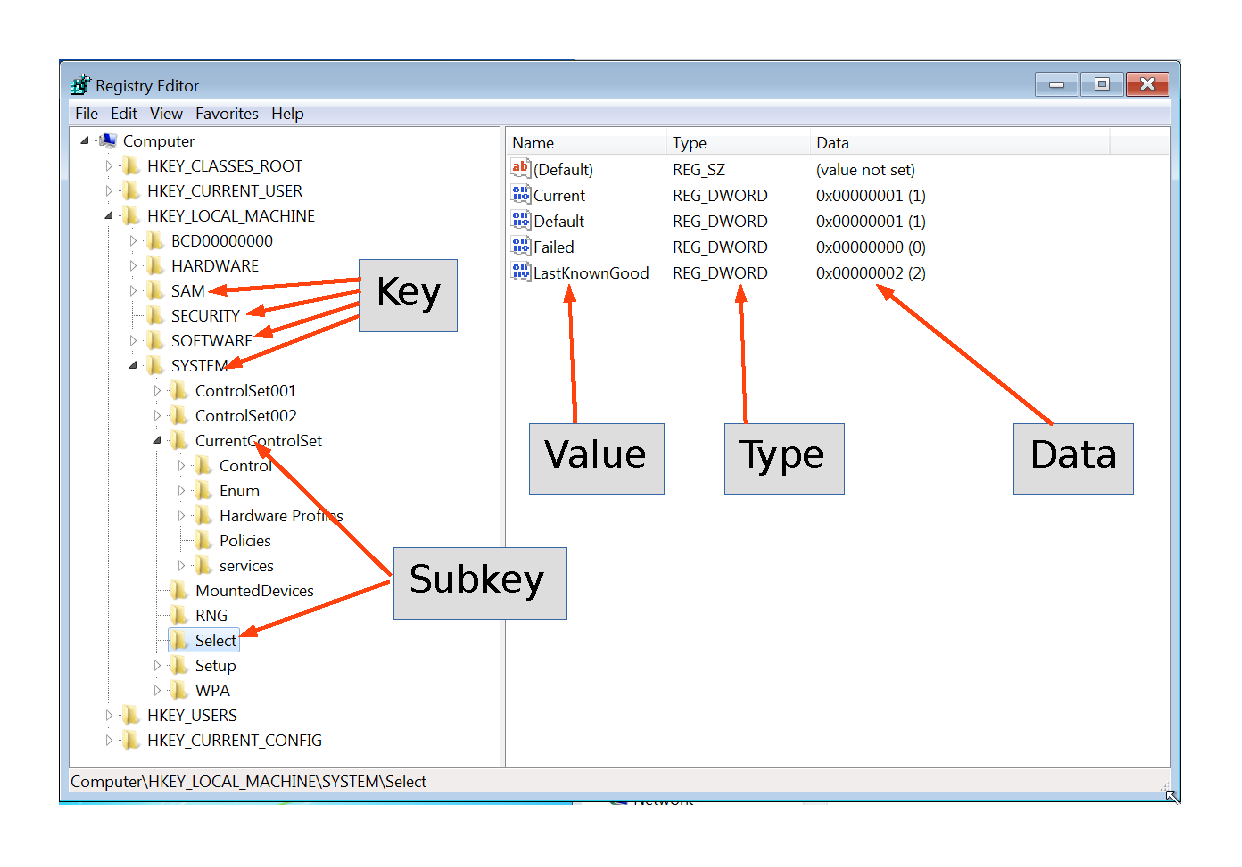
\includegraphics[scale=0.43]{images/nomenclature.pdf}
        \captionsetup{labelformat=empty,labelsep=none}
        \transparent{0.9}%
        \caption[]{\tiny Key data structures contains a last write time stamp}
    \end{figure}
\end{frame}


\begin{frame}[fragile]
  \frametitle{1.1 About: Windows Registry}
    \begin{itemize}
        \item Do you ever touch the Registry?
            \begin{itemize}
		\item \texttt{regedit.exe}
                \item Black Magic for many admins
		\item[] $\to$ Every user interacts with the Registry
		\item[]
            \end{itemize}
        \item Location of the hive files
            \begin{itemize}
                \item[] \begin{verbatim}%SystemRoot%\system32\config\end{verbatim}
                \item[] $\to$ \texttt{SAM, SECURITY, SYSTEM, SOFTWARE}
                \item[] \begin{verbatim}%UserProfile%\NTUSER.DAT\end{verbatim}
                \item[] \begin{verbatim}%UserProfile%\AppData\Local\Microsoft\Windows\UsrClass.dat\end{verbatim}
		\item[]
            \end{itemize}
        \item Timestamps $\to$ Timeline
    \end{itemize}
\end{frame}


\begin{frame}[fragile]
  \frametitle{1.2 Under the hood: Key Cell}
  \definecolor{light-gray}{gray}{0.70}
  \begin{lstlisting}[basicstyle=\tiny,escapechar=§]
     0000:  §\colorbox{light-gray}{a0ff ffff}§ 6e6b 2000  6f0f 0e3b b78d d101  ....nk .o..;....
     0010:  0200 0000 085e 0500  0000 0000 0000 0000  .....^..........
     0020:  ffff ffff ffff ffff  0200 0000 0021 0500  .............!..
     0030:  102e 0000 ffff ffff  0000 0000 0000 0000  ................
     0040:  1400 0000 1000 0000  0000 0000 0a00 0000  ................
     0050:  496e 7465 7266 6163  6573 0080 0200 0000  Interfaces......
  \end{lstlisting}
  \begin{lstlisting}[basicstyle=\tiny]
 Offsets:    0x00       0       4        Size
             0x04       4       2        Node ID
             0x06       6       2        Node type
             0x08       8       8        Last write time
                  ...      ...
             0x4c      76       2        Lenght of key name
             0x50      80     <76>       key name + padding
  \end{lstlisting}
  \begin{itemize}
      \item Exercise: Calculate the size of the key cell
      \begin{itemize}
          \item[] \texttt{a0 ff ff ff}
          \item[]
      \end{itemize}
      \item Exercise: Calculate the size of the key name
      \begin{itemize}
          \item[] \texttt{0a 00}
      \end{itemize}
  \end{itemize}
\end{frame}


\begin{frame}[fragile]
  \frametitle{1.2 Under the hood: Value Cell}
  \definecolor{light-gray}{gray}{0.70}
  \begin{lstlisting}[basicstyle=\tiny,escapechar=§]
     0000:                        §\colorbox{light-gray}{d8ff ffff}§ 766b 0d00          ....vk..
     0010:  0400 0080 0200 0000  0400 0000 0100 0000  ................
     0020:  4c61 7374 4b6e 6f77  6e47 6f6f 6400 0000  LastKnownGood...
  \end{lstlisting}
  \begin{lstlisting}[basicstyle=\tiny]
 Offset:     0x00       0       4        Size
             0x04       4       2        Node ID
             0x06       6       2        Value name length
             0x08       8       4        Data lenght
             0x0c      12       4        Data offset
             0x10      16       4        value typw
  \end{lstlisting}
  \begin{itemize}
      \item Exercise: Calculate the size of the value cell
      \begin{itemize}
          \item[] \texttt{d8 ff ff ff}
          \item[]
      \end{itemize}
      \item Exercise: Calculate the size of the value name length
      \begin{itemize}
          \item[] \texttt{0d 00}
      \end{itemize}
  \end{itemize}
\end{frame}


\begin{frame}[fragile]
  \frametitle{1.3 Hive files}
   \begin{itemize}
       \item[]
   \begin{itemize}
      \item SAM
      \begin{itemize}
          \item Local users
      \end{itemize}
      \item Security
      \begin{itemize}
          \item Audit settings
          \item Machine, domain SID
      \end{itemize}
      \item System
      \begin{itemize}
          \item General system configuration
          \item Networking, Auto run
          \item Program execution
          \item USB devices
       \end{itemize}
      \item Software
      \begin{itemize}
          \item Windows version, Profiles list
          \item Networking, Auto run
          \item Shell extensions, Browser helper objects
          \item Scheduled Tasks
          \item Program execution
      \end{itemize}
   \end{itemize}
   \end{itemize}
\end{frame}


\begin{frame}[fragile]
  \frametitle{1.3 Hive files}
    \begin{itemize}
        \item Windows XP:
        \item[] \begin{verbatim}C:\Documents and Settings\<username>\NTUSER.DAT\end{verbatim}
        \item[] \begin{verbatim}C:\Documents and Settings\<username>\Local Settings\\end{verbatim}
        \item[] \begin{verbatim}   Application Data\Microsoft\Windows\UsrClass.dat\end{verbatim}
        \item[]
        \item Windows Vista and above:
        \item[] \begin{verbatim}C:\Users\<user>\NTUSER.DAT\end{verbatim}
        \item[] \begin{verbatim}C:\Users\<user>\AppData\Local\Microsoft\Windows\\end{verbatim}
        \item[] \begin{verbatim}   UsrClass.dat\end{verbatim}
        \item[]
        \item \begin{verbatim}C:\Windows\inf\setupapi.log\end{verbatim}
    \end{itemize}
\end{frame}


\begin{frame}[fragile]
  \frametitle{1.4 RegRipper}
  \begin{itemize}
      \item Extract specific key values
  \begin{lstlisting}[basicstyle=\tiny]
$ rip.pl -p compname -r SYSTEM
	ComputerName    = WIN7WS
	TCP/IP Hostname = Win7WS
  \end{lstlisting}
      \item Alternative method
  \begin{lstlisting}[basicstyle=\tiny]
$ wine rip.exe -p compname -r SYSTEM
	ComputerName    = WIN7WS
	TCP/IP Hostname = Win7WS
  \end{lstlisting}
      \item RegRipper plugins
  \begin{lstlisting}[basicstyle=\tiny]
$ ls -l /usr/share/regripper/plugins | wc -l
	397
  \end{lstlisting}
      \item Ripping hive files with profiles
  \begin{lstlisting}[basicstyle=\tiny]
$ rip.exe -f sam -r SAM > out/sam.txt
$ rip.exe -f security -r SECURITY > out/security.txt
$ rip.exe -f system -r SYSTEM > out/system.txt
$ rip.exe -f software -r SOFTWARE > out/software.txt
$ rip.exe -f ntuser -r NTUser.dat > out/ntuser.txt
$ rip.exe -f usrclass -r UsrClass.dat > out/userClass.txt
  \end{lstlisting}
  \end{itemize}
\end{frame}


\begin{frame}[fragile]
  \frametitle{1.5 RegRipper: Exercise}
  \begin{enumerate}
      \item Extract Hive files from invected PC
      \item Rip them with RegRipper profiles
      \item Collect important general information
      \item Try to find incident related artefacts
      \item Add the information to report
  \end{enumerate}
\end{frame}


\begin{frame}[fragile]
  \frametitle{1.6 Examples: System Hive}
   \begin{itemize}
      \item Computer name
      \item Services
      \item Network configuration
      \item Devices / USB device
      \begin{itemize}
	  \item \texttt{\scriptsize{SYSTEM/ControlSet001/Enum/USBStor}}
	  \item[] $\to$ Device class ID
	  \item[] $\to$ Unique instance ID (SN)
	  \item[] $\to$ First connect time stamp
	  \item[]
	  \item \texttt{\scriptsize{SYSTEM/ControlSet001/Enum/USB}}
	  \item[] $\to$ Last connect time stamp
	  \item[]
	  \item \texttt{\scriptsize{SYSTEM/MountedDevices}}
	  \item[] $\to$ Voume GUID
	  \item[] $\to$ Mount Point
	  \item[]
      \end{itemize}
   \end{itemize}
\end{frame}


\begin{frame}[fragile]
  \frametitle{1.7 Examples: Software Hive}
   \begin{itemize}
      \item OS version \& configuration
      \item Applications installed \& uninstalled
      \item Application configuration system wide
      \item Drivers
      \item Network lists \& interfaces
      \item User profiles
      \item Schedules Tasks
      \item Auto start
      \item Example: Get Windows version:
      \begin{itemize}
	  \item \texttt{\scriptsize{wine rip.exe -p winver -r SOFTWARE}}
	  \item[]
      \end{itemize}
   \end{itemize}
\end{frame}


\begin{frame}[fragile]
  \frametitle{1.7 Examples: User Hive}
   \begin{itemize}
      \item OS configuration user related
      \item Applications installed \& uninstalled
      \item Application configuration user related
      \item Auto start
      \begin{itemize}
          \item Run
              \begin{itemize}
                  \item Executed at user login
                  \item Provide \(malware\) persistence
                  \item No admin privileges required
              \end{itemize}
          \item RunOnce
          \item Legacy and other AutoStart
              \begin{itemize}
		      \item \texttt{\scriptsize{/Software/Microsoft/Windows/CurrentVersion/Policies/Explorer/Run/}}
		      \item \texttt{\scriptsize{/Software/Microsoft/Windows NT/CurrentVersion/Windows/'load','run'}}
              \end{itemize}
          \item Much more auto start loctions... 
      \end{itemize}
   \end{itemize}
\end{frame}


\begin{frame}[fragile]
  \frametitle{1.7 Examples: User Hive}
   \begin{itemize}
      \item WordWheelQuery
        \begin{itemize}
           \item User search on localhost
           \item MRU List
	   \item[] $\to$ Consider VSS for histrorical data
        \end{itemize}
      \item Shell Bags
        \begin{itemize}
          \item User preferences for diplaying Explorer windows
          \item Postion, size, view, icon
	  \item[] $\to$ Folders accessed by the user 
        \end{itemize}
      \item UserAssist
        \begin{itemize}
	  \item User activities
            \begin{itemize}
	      \item Double-click icon
              \item Launch application from 'START Menu'
            \end{itemize}
	  \item Values stored:
            \begin{itemize}
              \item Path, Run-Count, FileTime last access
              \item ROT-13
            \end{itemize}
        \end{itemize}
   \end{itemize}
\end{frame}


\begin{frame}[fragile]
  \frametitle{1.7 Examples: User Hive}
   \begin{itemize}
      \item MUICache
        \begin{itemize}
          \item Program execution incl. called from CMD
        \end{itemize}
      \item RecentDocs
        \begin{itemize}
          \item[] Example: '.png' files
          \begin{lstlisting}[basicstyle=\tiny]
Software\Microsoft\Windows\CurrentVersion\Explorer\RecentDocs\.png
LastWrite Time Fri Jan 12 15:00:52 2018 (UTC)
MRUListEx = 3,2,0,1
  3 = photo-123.png
  2 = paint.png
  0 = face.png
  1 = flower.png
          \end{lstlisting}
        \end{itemize}
      \item Common Dialogs
        \begin{itemize}
          \item[] Example: 'Open' and 'Save As...'
          \begin{lstlisting}[basicstyle=\tiny]
OpenSavePidlMRU\exe
LastWrite Time: Tue Jul  5 14:40:46 2016
Note: All value names are listed in MRUListEx order.

  Users\avast_free_antivirus_setup_online.exe
  Users\Thunderbird Setup 45.1.1.exe
  Users\Firefox Setup Stub 47.0.1.exe
          \end{lstlisting}
        \end{itemize}
   \end{itemize}
\end{frame}


\begin{frame}[fragile]
  \frametitle{1.8 Exercises}
  \begin{lstlisting}[basicstyle=\tiny]
Identify computer name:



What services start during system boot:



Gather list of network connected:



What network cards are configured:



Get list of user profiles:



Get Windows version:



Detect Auto Start applications from the NTUser.dat hive:

.
  \end{lstlisting}
\end{frame}


\begin{frame}[fragile]
  \frametitle{1.8 Exercises}
  \begin{lstlisting}[basicstyle=\tiny]
Identify computer name:
          $ wine rip.exe -p compname -r SYSTEM


What services start during system boot:
          $ wine rip.exe -p services -r SYSTEM


Gather list of network connected:
          $ wine rip.exe -p networklist -r SOFTWARE


What network cards are configured:
          $ wine rip.exe -p networkcards -r SOFTWARE


Get list of user profiles:
          $ wine rip.exe -p profilelist -r SOFTWARE


Get Windows version:
          $ wine rip.exe -p winver -r SOFTWARE


Detect Auto Start applications from the NTUser.dat hive:
          $ wine rip.exe -p user_run -r JohnNTUser.DAT
.
  \end{lstlisting}
\end{frame}






%
% This work is licensed under a Creative Commons Attribution-ShareAlike 4.0 International License.
% http://creativecommons.org/licenses/by-sa/4.0/
%

% DO NOT COMPILE THIS FILE DIRECTLY!
% This is included by the other .tex files.


\begin{frame}
    
\includegraphics[scale=.3]{images/logo-circl-Forensics.png}
    \begin{itemize}
        \item[]
        \item[]
        \item[] 2. Windows Event Logs
    \end{itemize}
\end{frame}


\begin{frame}[fragile]
  \frametitle{2.1 Inroduction}
    \begin{itemize}
        \item Up to Windows XP
            \begin{itemize}
                \item Binary Event Log file format
                \item Mainly 3 categories:
                \begin{itemize}
			\item[] Security:  \texttt{secevent.evt}
			\item[] System:  \texttt{sysevent.evt}
			\item[] Application:  \texttt{appevent.evt}
			\item[] ... maybe some server service specific
			\item[]
                \end{itemize}
            \end{itemize}
        \item Beginning with Vista
            \begin{itemize}
                \item New binary XML format
		\item New extension: \texttt{.evtx}
		\item Location: \texttt{/Windows/System32/winevt/Logs/}
                \item Many more files:
                \begin{itemize}
			\item[] \texttt{Security.evtx}
			\item[] \texttt{System.evtx}
			\item[] \texttt{Application.evtx}
			\item[] $\to$ 120 files ++
                \end{itemize}
            \end{itemize}
    \end{itemize}
\end{frame}


\begin{frame}[fragile]
  \frametitle{2.1 Inroduction}
    \begin{itemize}
        \item Advantage
            \begin{itemize}
                \item Full fledged logging
                \item Logon Success: Importand events are logged
                \item Detailed importand information
		\item[] 
            \end{itemize}
        \item Disadvantage
            \begin{itemize}
                \item Cover only a limited period of time
                \item Logon Fail: Importand events are not logged per default
                \item Much information, hard to read
		\item[]
            \end{itemize}
        \item Always interesting
            \begin{itemize}
                \item Logon / Logoff
                \item System boot
                \item Services started
		\item[]
            \end{itemize}
    \end{itemize}
\end{frame}


\begin{frame}[fragile]
  \frametitle{2.2 Example: Logon event}
    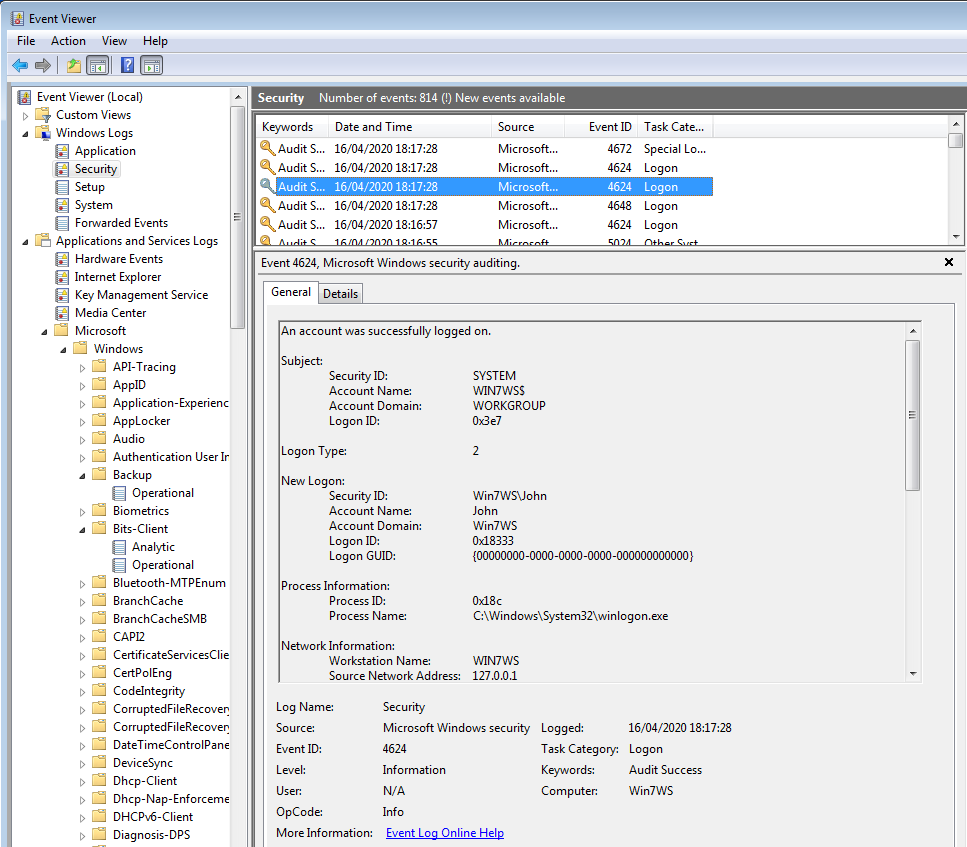
\includegraphics[scale=0.24]{images/evtx.png}
\end{frame}


\begin{frame}[fragile]
  \frametitle{2.3 In Forensics}
    \begin{itemize}
        \item Get support online:
            \begin{itemize}
                \item Microsoft TechNet
		\item \url{https://www.ultimatewindowssecurity.com/securitylog/encyclopedia/}
		\item \url{http://eventid.net/}
            \end{itemize}
        \item Review logging policies
  \begin{lstlisting}[basicstyle=\tiny]
$ rip.pl -r SECURITY -p auditpol
.....
ystem:Other System Events                         S/F  
Logon/Logoff:Logon                                 S    
Logon/Logoff:Logoff                                S    
Logon/Logoff:Account Lockout                       S    
Logon/Logoff:IPsec Main Mode                       N    
Logon/Logoff:IPsec Quick Mode                      S    
Logon/Logoff:IPsec Extended Mode                   N    
Logon/Logoff:Special Logon                         N    
Logon/Logoff:Other Logon/Logoff Events             N    
Logon/Logoff:Network Policy Server                 S/F  
Object Access:File System                          N    
.....
  \end{lstlisting}
    \end{itemize}
\end{frame}


\begin{frame}[fragile]
  \frametitle{12.4 Explore and extract evtx}
    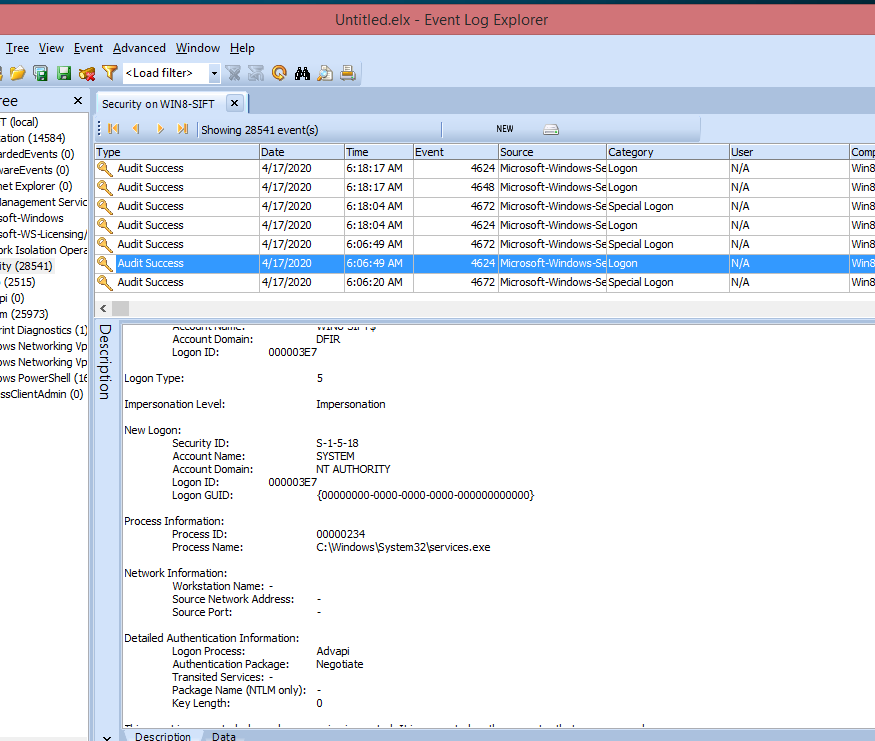
\includegraphics[scale=0.27]{images/evtx2.png}
\end{frame}


\begin{frame}[fragile]
  \frametitle{2.5 Example}
    \begin{itemize}
        \item Logon Success
  \begin{lstlisting}[basicstyle=\tiny]
$ evtxexport Security.evtx | less
.....
Event number          : 668
Written time          : Apr 15, 2019 12:58:33.650031000 UTC
Event level           : Information (0)
Computer name         : Win7WS
Source name           : Microsoft-Windows-Security-Auditing
Event identifier      : 0x00001210 (4624)
Number of strings     : 20
String: 1             : S-1-5-18
String: 2             : WIN7WS$
String: 3             : WORKGROUP
String: 4             : 0x00000000000003e7
String: 5             : S-1-5-21-3408732720-2018246097-660081352-1000
String: 6             : John
String: 7             : Win7WS
String: 9             : 2
.....
String: 17            : 0x0000018c
String: 18            : C:\Windows\System32\winlogon.exe
String: 19            : 127.0.0.1
  \end{lstlisting}
        \item Logon Fail
  \begin{lstlisting}[basicstyle=\tiny]
$ evtxexport Security.evtx | grep 4625
  \end{lstlisting}
    \end{itemize}
\end{frame}


\begin{frame}[fragile]
  \frametitle{2.5 Example}
    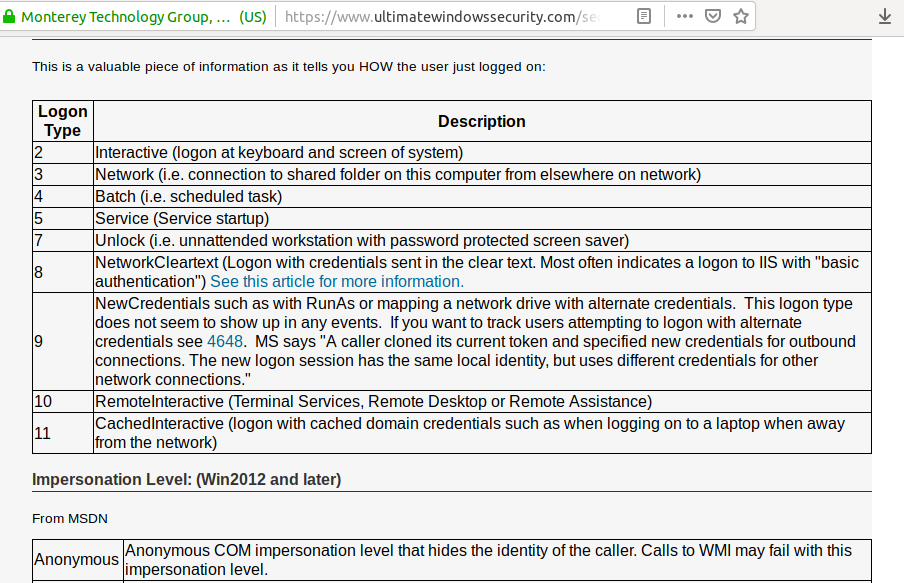
\includegraphics[scale=0.4]{images/f14_logonType.png}
\end{frame}


\begin{frame}[fragile]
  \frametitle{2.6 Other log files}
    \begin{itemize}
	\item \texttt{/Windows/setuplog.txt}
        \begin{itemize}
            \item Untill WinXP, when Windows is installed
        \end{itemize}
	\item \texttt{/Windows//Debug/netsetup.log}
        \begin{itemize}
            \item Untill WinXP, when Windows is installed
        \end{itemize}
	\item \texttt{/Windows/setupact.log}
        \begin{itemize}
            \item Graphical part of setup process
  \begin{lstlisting}[basicstyle=\tiny]
2019-04-05 11:39:56, Info  CBS Starting the TrustedInstaller main loop.
2019-04-05 11:39:56, Info  CBS TrustedInstaller service starts successfully.
2019-04-05 11:39:56, Info  CBS Setup in progress, aborting startup processing checks.
2019-04-05 11:39:56, Info  CBS Startup processing thread terminated normally
    \end{lstlisting}
	\end{itemize}
	\item \texttt{/Windows/setupapi.log}
  \begin{lstlisting}[basicstyle=\tiny]
/Windows/inf/setupapi.dev.log
/Windows/inf/setupapi.app.log
/Windows/inf/setupapi.offline.log
    \end{lstlisting}
	\item \texttt{/Windows/Tasks/SCHEDLGU.TXT}
        \begin{itemize}
            \item Task Scheduler Log
	\end{itemize}
    \end{itemize}
\end{frame}


\begin{frame}[fragile]
  \frametitle{2.7 Exercise: Event Log}
    \begin{enumerate}
        \item Which .evtx files could be interesting for forensics?
        \item Extract promising .evtx files
	\item Try tools like \texttt{evtx\_dump.py} to read some logs
        \item Find general information like:
        \begin{itemize}
            \item What time the system boot up
            \item What user was logged on
            \item Was there much user activity before infection
            \item What time the system shut down
        \end{itemize}
        \item Search for other incident related artefacts in .evtx files
        \item Are artefacts within the other log files?
    \end{enumerate}
\end{frame}






%
% This work is licensed under a Creative Commons Attribution-ShareAlike 4.0 International License.
% http://creativecommons.org/licenses/by-sa/4.0/
%

% DO NOT COMPILE THIS FILE DIRECTLY!
% This is included by the other .tex files.


\begin{frame}
    
\includegraphics[scale=.3]{images/logo-circl-Forensics.png}
    \begin{itemize}
        \item[]
        \item[]
        \item[] 3. Other Sources of Information
    \end{itemize}
\end{frame}


\begin{frame}[fragile]
  \frametitle{3.1 Recycle Bin - User support to undelete}
    \begin{itemize}
        \item Files move to Recycle Bin:
            \begin{itemize}
                \item Moved by mouse
		\item Right click: \texttt{Delete}
            \end{itemize}
        \item Not move to Recycle Bin:
            \begin{itemize}
		    \item Right click: \texttt{Delete + SHIFT}
		    \item Command line: \texttt{del}
		\item Files on network shares
            \end{itemize}
        \item NukeOnDelete
            \begin{itemize}
		    \item \texttt{HKEY\_USERS/\_UUID\_/Software/Microsoft/Windows/CurrentVers}
		    \item[]\texttt{ion/Explorer/BitBucket/Volume/\{\_Volume ID\_\}/NukeOnDelete}
                    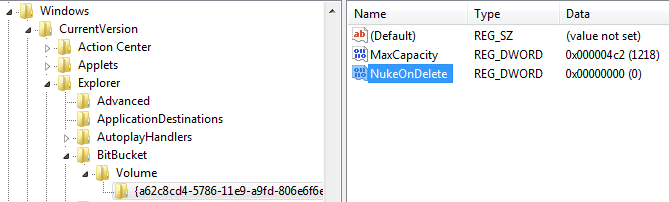
\includegraphics[scale=.3]{images/nukeOD.png}
            \end{itemize}
    \end{itemize}
\end{frame}


\begin{frame}[fragile]
  \frametitle{3.1 Recycle Bin - Life-Investigate}
    \begin{itemize}
        \item Play script: \texttt{TextFile.txt} 
            \begin{itemize}
		\item 2019-04-30 17:31:57 UTC+2:  Born
		\item 2019-04-30 17:34:44 UTC+2:  Content Modified
		\item 2019-04-30 17:35:32 UTC+2:  Deleted
		\item[]
            \end{itemize}
        \item Analyze Recycle.Bin:
        \item[] 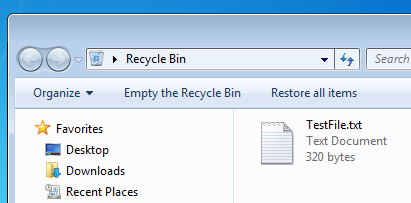
\includegraphics[scale=.45]{images/f15_recycle.png}
    \end{itemize}
\end{frame}


\begin{frame}[fragile]
  \frametitle{3.1 Recycle Bin - Forensics}
    \begin{itemize}
        \item Play script: \texttt{TextFile.txt} 
            \begin{itemize}
		\item 2019-04-30 17:31:57 UTC+2:  Born
		\item 2019-04-30 17:34:44 UTC+2:  Content Modified
		\item 2019-04-30 17:35:32 UTC+2:  Deleted
		\item[]
            \end{itemize}
        \item Analyze \texttt{Recycle.Bin} directory:
  \begin{lstlisting}[basicstyle=\tiny]
/$Recycle.Bin/S-1-5-21-3408732720-2018246097-660081352-1000/
	129 Apr  5 11:46  desktop.ini
	544 Apr 30 17:35 '$IOMHI9A.txt'
	320 Apr 30 17:34 '$ROMHI9A.txt'

strings \$ROMHI9A.txt 
		Test File
		=========
	This is a test file. It is just created to test Forensic
	Artifacts for the 'Recycle Bin'.
	.....

strings -el \$IOMHI9A.txt 
	C:\Users\John\Documents\recycleTest\TestFile.txt
  \end{lstlisting}
    \end{itemize}
\end{frame}


\begin{frame}[fragile]
  \frametitle{3.1 Recycle Bin - Forensics}
    \begin{itemize}
        \item Play script: \texttt{TextFile.txt} 
            \begin{itemize}
		\item 2019-04-30 17:31:57 UTC+2:  Born
		\item 2019-04-30 17:34:44 UTC+2:  Content Modified
		\item 2019-04-30 17:35:32 UTC+2:  Deleted
		\item[]
            \end{itemize}
        \item Analyze \texttt{Recycle.Bin} directory:
  \begin{lstlisting}[basicstyle=\tiny]
Fri Apr 05 2019 11:46:49
     328 m.c.      57-144-1 /$Recycle.Bin
     376 ...b    9632-144-1 /$Recycle.Bin/S-1-5-21- ..... -1000
     129 m.cb    9634-128-1 /$Recycle.Bin/S-1-5-21- ..... -1000/desktop.ini

Tue Apr 30 2019 17:31:57
     320 ...b   47164-128-1 /$Recycle.Bin/S-1-5-21- ..... -1000/$ROMHI9A.txt

Tue Apr 30 2019 17:34:44
     320 ma..   47164-128-1 /$Recycle.Bin/S-1-5-21- ..... -1000/$ROMHI9A.txt

Tue Apr 30 2019 17:35:32
     544 macb   44155-128-1 /$Recycle.Bin/S-1-5-21- ..... -1000/$IOMHI9A.txt
      48 mac.   47022-144-1 /Users/John/Documents/recycleTest
     320 ..c.   47164-128-1 /$Recycle.Bin/S-1-5-21- ..... -1000/$ROMHI9A.txt
     376 mac.    9632-144-1 /$Recycle.Bin/S-1-5-21- ..... -1000
  \end{lstlisting}
    \end{itemize}
\end{frame}


\begin{frame}[fragile]
  \frametitle{3.1 Recycle Bin - Exercise}
    \begin{itemize}
	    \item[] Invetigate extension of an index file \texttt{\$I.....} for binary file:
    \end{itemize}
    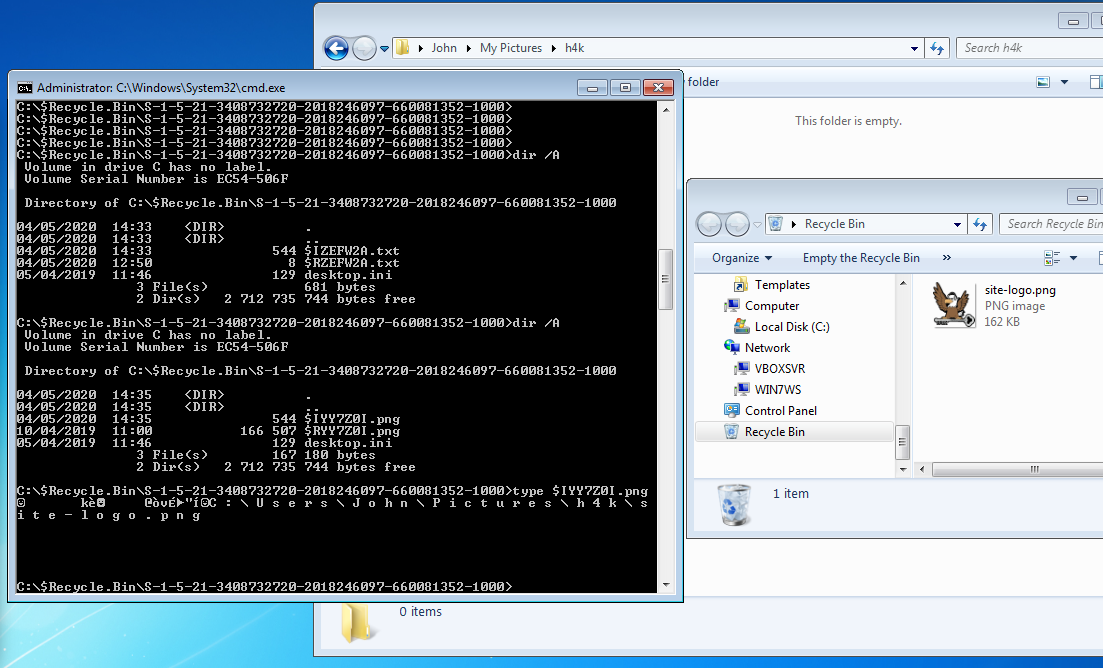
\includegraphics[scale=.27]{images/recycleEx.png}
\end{frame}


\begin{frame}[fragile]
  \frametitle{3.2 LNK Files}
    \begin{itemize}
        \item Provide information about files accessed
        \begin{itemize}
            \item Local
            \item Network shares
            \item Appached devices
        \end{itemize}
    \end{itemize}
  \begin{lstlisting}[basicstyle=\tiny]
Thu May 02 2019 14:54:02
     280 ...b       43701-144-1 /Users/John/Documents/prefetchTest
  
Thu May 02 2019 14:54:28
      66 macb       43702-128-1 /Users/John/Documents/prefetchTest/
      				PreFetchTest.txt
    2779 macb       43716-128-4 /Users/John/AppData/Roaming/Microsoft/
    				Windows/Recent/PreFetchTest.txt.lnk
    1573 macb       43922-128-4 /Users/John/AppData/Roaming/Microsoft/
    				Windows/Recent/prefetchTest.lnk
  \end{lstlisting}
\end{frame}


\begin{frame}[fragile]
  \frametitle{3.2 LNK Files}
    \begin{itemize}
        \item Provide information about files accessed
        \begin{itemize}
            \item Local
            \item Network shares
            \item Appached devices
        \end{itemize}
    \end{itemize}
  \begin{lstlisting}[basicstyle=\tiny]
exiftool PreFetchTest.txt.lnk

	...
	Create Date         : 2019:05:02 14:54:28+02:00
	Access Date         : 2019:05:02 14:54:28+02:00
	Modify Date         : 2019:05:02 14:54:28+02:00
	Target File Size    : 66
	Icon Index          : (none)
	Run Window          : Normal
	Hot Key             : (none)
	Drive Type          : Fixed Disk
	Volume Label        :
	Local Base Path     : C:\Users\John\Documents\prefetchTest\
				PreFetchTest.txt
	...
  \end{lstlisting}
\end{frame}


\begin{frame}[fragile]
  \frametitle{3.3 XP Restore Points}
    \begin{itemize}
        \item Backup of:
        \begin{itemize}
	    \item Critical system files
	    \item Registry partially
            \item Local user profiles
            \item But NO user data!
        \end{itemize}
        \item Created automatically:
        \begin{itemize}
            \item Every 24 hours
            \item Windows Update
	    \item Installation of applications incl. driver
            \item Manually
        \end{itemize}
        \item For user: Useful to recover a broken system
        \item For analyst:
        \begin{itemize}
	    \item \texttt{rp.log}
            \item Description of the cause
            \item Time stamp
            \item State of the system at different times
        \end{itemize}
    \end{itemize}
\end{frame}


\begin{frame}[fragile]
  \frametitle{3.4 VSS - Volume Shadow Copy Service}
    \begin{itemize}
	    \item Backup Service
            \begin{itemize}
	         \item System files
	         \item User data files
	         \item Operates on block level
            \end{itemize}
	    \item On live system
            \begin{itemize}
	         \item Run CMD as administrator
  \begin{lstlisting}[basicstyle=\tiny]
>vssadmin list shadows /for=c:/
vssadmin 1.1 - Volume Shadow Copy Service administrative command-line tool
(C) Copyright 2001-2005 Microsoft Corp.

Contents of shadow copy set ID: {33eb3a7b-6d03-4045-aa70-37b714d49c72}
   Contained 1 shadow copies at creation time: 10/04/2019 16:06:30
      Shadow Copy ID: {34d9910b-ac1d-4b10-b282-89dde217d0fb}
         Original Volume: (C:)\\?\Volume{a62c8cd4-5786-11e9-a9fd-806e6f6e6963}\
         Shadow Copy Volume: \\?\GLOBALROOT\Device\HarddiskVolumeShadowCopy1
         Originating Machine: Win7WS
         Service Machine: Win7WS
         Provider: 'Microsoft Software Shadow Copy provider 1.0'
         Type: ClientAccessibleWriters
         Attributes: Persistent, Client-accessible, No auto release, Differential,
	 Auto recovered
  \end{lstlisting}
            \end{itemize}
  \end{itemize}
\end{frame}


\begin{frame}[fragile]
  \frametitle{3.4 VSS - Configuration}
	    \begin{itemize}
		    \item[] \scriptsize{\texttt{HKEY\_LOCAL\_MACHINE/SYSTEM/CurrentControlSet/services/VSS}}
		    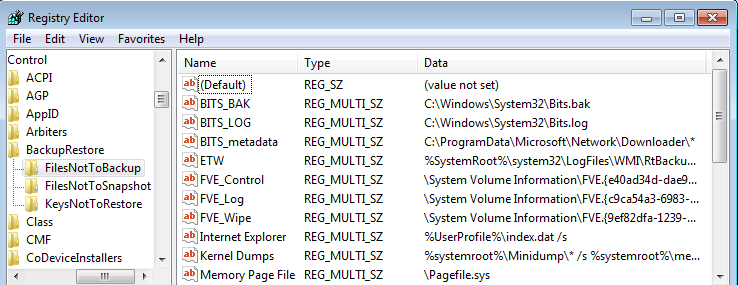
\includegraphics[scale=.3]{images/VSSConfig2.png}
		    \item[]
	    \item[] \scriptsize{\texttt{HKEY\_LOCAL\_MACHINE/SYSTEM/CurrentControlSet/Control/BackupRestore}}
		    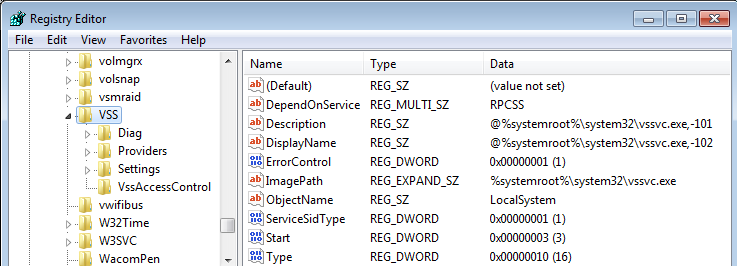
\includegraphics[scale=.3]{images/VSSConfig.png}
            \end{itemize}
\end{frame}


\begin{frame}[fragile]
  \frametitle{3.4 VSS - Analysis}
    \begin{itemize}
	    \item[] Analyze disk image
  \begin{lstlisting}[basicstyle=\tiny]
vshadowinfo -o $((512*206848)) 8d34ce.raw 

    Volume Shadow Snapshot information:
	Number of stores:	1

    Store: 1
	Identifier		: 237c8de3-5b99-11e9-9925-080027062798
	Shadow copy set ID	: 33eb3a7b-6d03-4045-aa70-37b714d49c72
	Creation time		: Apr 10, 2019 14:06:30.365699200 UTC
	Shadow copy ID		: 34d9910b-ac1d-4b10-b282-89dde217d0fb
	Volume size		: 11 GiB (12777947136 bytes)
	Attribute flags		: 0x0042000d
  \end{lstlisting}
	    \item[] Mounting VSC: A 2 step approach
  \begin{lstlisting}[basicstyle=\tiny]
sudo vshadowmount -o $((512*206848)) 8d34ce.raw /mount/vss/

sudo ls -l /mount/vss/
	-r--r--r-- 1 root root 12777947136 Jan  1  1970 vss1

sudo file /mount/vss/vss1
	/mount/vss/vss1: DOS/MBR boot sector, code offset 0x52+2, OEM-ID "NTFS 

sudo mount -o ro /mount/vss/vss1 /mnt/
  \end{lstlisting}
  \end{itemize}
\end{frame}


\begin{frame}[fragile]
  \frametitle{3.5 Prefetch Files \& SuperFetch}
    \begin{itemize}
        \item Boot prefetching for all Windows
	\item Application prefetching since XP
        \begin{itemize}
            \item Monitor an application when it starts
            \item Collect information about all resources needed
            \item Wait 10sec after application started
	    \item[] $\to$ Know where to find the resources
            \item[] $\to$ Better performance: App launch faster
            \item[] $\to$ Better user experience
        \end{itemize}
	\item Forensics value:
        \begin{itemize}
            \item Proof an application was started
            \begin{itemize}
                \item Secondary artifact
                \item Created by the OS
                \item Not deleted by the attacker
            \end{itemize}
            \item Even if the application don't exists anymore
            \item And more .....
        \end{itemize}
    \end{itemize}
\end{frame}


\begin{frame}[fragile]
  \frametitle{3.5 Prefetch Files \& SuperFetch}
    \begin{itemize}
        \item Elements of the file name at \texttt{/Windows/Prefetch}
        \begin{itemize}
            \item Application name
            \item One way hash of path to the application
	    \item File extension: \texttt{.pf}
        \end{itemize}
        \item Example: File system time line
  \begin{lstlisting}[basicstyle=\tiny]
Thu May 02 2019 14:52:40
    179712 .a..      10940-128-3 /Windows/notepad.exe

Thu May 02 2019 14:52:50
        56 mac.      42729-144-6 /Windows/Prefetch
     16280 macb      43700-128-4 /Windows/Prefetch/NOTEPAD.EXE-D8414F97.pf
  \end{lstlisting}
        \item Information found inside a Prefetch file:
        \begin{itemize}
            \item Run count: How often launched
            \item Last time executed
            \item Application name incl. parameter
            \item Path to application and resources
        \end{itemize}
    \end{itemize}
\end{frame}


\begin{frame}[fragile]
  \frametitle{3.5 Prefetch Files \& SuperFetch}
    \begin{itemize}
        \item Parsing a Prefetch file
  \begin{lstlisting}[basicstyle=\tiny]
prefetch.py -f NOTEPAD.EXE-D8414F97.pf

	Executable Name: NOTEPAD.EXE
	Run count: 1
	Last Executed: 2019-05-02 12:52:40.339584

	Resources loaded:
	1:    \DEVICE\HARDDISKVOLUME2\WINDOWS\SYSTEM32\NTDLL.DLL
	2:    \DEVICE\HARDDISKVOLUME2\WINDOWS\SYSTEM32\KERNEL32.DLL
	3:    \DEVICE\HARDDISKVOLUME2\WINDOWS\SYSTEM32\APISETSCHEMA.DLL
	4:    \DEVICE\HARDDISKVOLUME2\WINDOWS\SYSTEM32\KERNELBASE.DLL
	.....
	.....
  \end{lstlisting}
        \item Additional benefits like:
        \begin{itemize}
            \item User folder where the malware got executed
            \item Compare Run count of different VSS could
	    \item[] $\to$ Behavior of user
        \end{itemize}
    \end{itemize}
\end{frame}


\begin{frame}[fragile]
  \frametitle{3.6 Jump Lists}
    \begin{itemize}
        \item Since Windows 7
        \item Recently opened documents of an application
	\item Similar \texttt{RecentDocs} Registry Key
	\item[]
        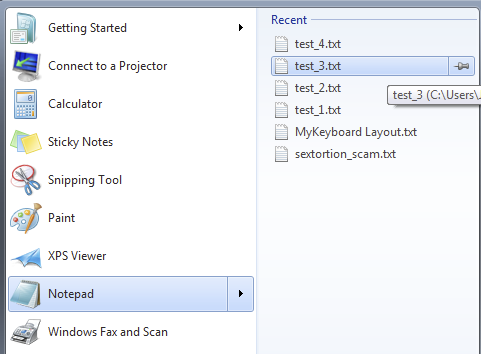
\includegraphics[scale=.3]{images/jl.png}
        \item Rotate or Pin
	\item \scriptsize{\texttt{AppData/Roaming/Microsoft/Windows/Recent/AutomaticDestinations}}
        \item[]
    \end{itemize}
\end{frame}


\begin{frame}[fragile]
  \frametitle{3.6 Jump Lists}
    \begin{itemize}
        \item Jump List file names start with 16 hex characters
	\item File names end with \texttt{.automaticDextinations-ms}
	\item[]
  \begin{lstlisting}[basicstyle=\tiny]
C:> dir \Users\John\AppData\Roaming\Microsoft\Windows\Recent\AutomaticDestinations

04/05/2020  12:50            33 792 1b4dd67f29cb1962.automaticDextinations-ms
14/06/2019  16:43             4 608 28c8b86deab549a1.automaticDextinations-ms
10/04/2019  14:32            29 696 6824f4a902c78fbd.automaticDextinations-ms
10/04/2020  14:12             9 216 7e4dca80246863e3.automaticDextinations-ms
04/05/2020  12:50             8 704 918e0ecb43d17e23.automaticDextinations-ms
10/04/2019  14:30             3 072 b74736c2bd8cc8a5.automaticDextinations-ms
09/04/2019  14:43             6 144 de48a32edcbe79e4.automaticDextinations-ms
  \end{lstlisting}
	\item Each Hex value correspond to an application
	\item \texttt{918e0ecb43d17e23 = Notepad.exe}
	\item Hex values are fixed world wide
        \item Search for Jump List IDs
    \end{itemize}
\end{frame}


\begin{frame}[fragile]
  \frametitle{3.6 Jump Lists}
    \begin{itemize}
        \item Exercise: Identify applications
  \begin{lstlisting}[basicstyle=\tiny]
$ cd JumpLists/AutomaticDestinations/
$ ll

    1b4dd67f29cb1962.automaticDestinations-ms --> 
    28c8b86deab549a1.automaticDestinations-ms --> 
    6824f4a902c78fbd.automaticDestinations-ms --> 
    7e4dca80246863e3.automaticDestinations-ms --> 
    918e0ecb43d17e23.automaticDestinations-ms --> 
    b74736c2bd8cc8a5.automaticDestinations-ms --> 
    de48a32edcbe79e4.automaticDestinations-ms --> 
  \end{lstlisting}
	\item Exercise: Analyze the Notepad Jump List file
  \begin{lstlisting}[basicstyle=\tiny]










-
  \end{lstlisting}
    \end{itemize}
\end{frame}


\begin{frame}[fragile]
  \frametitle{3.6 Jump Lists}
    \begin{itemize}
        \item Exercise: Identify applications
  \begin{lstlisting}[basicstyle=\tiny]
$ cd JumpLists/AutomaticDestinations/
$ ll

    1b4dd67f29cb1962.automaticDestinations-ms --> Windows Explorer
    28c8b86deab549a1.automaticDestinations-ms --> Internet Explorer 8
    6824f4a902c78fbd.automaticDestinations-ms --> Firefox 64.x
    7e4dca80246863e3.automaticDestinations-ms --> Control Panel
    918e0ecb43d17e23.automaticDestinations-ms --> Notepad (32-bit)
    b74736c2bd8cc8a5.automaticDestinations-ms --> WinZip
    de48a32edcbe79e4.automaticDestinations-ms --> Acrobat Reader 15.x
  \end{lstlisting}
	\item Exercise: Analyze the Notepad Jump List file
  \begin{lstlisting}[basicstyle=\tiny]










-
  \end{lstlisting}
    \end{itemize}
\end{frame}


\begin{frame}[fragile]
  \frametitle{3.6 Jump Lists}
    \begin{itemize}
        \item Exercise: Identify applications
  \begin{lstlisting}[basicstyle=\tiny]
$ cd JumpLists/AutomaticDestinations/
$ ll

    1b4dd67f29cb1962.automaticDestinations-ms --> Windows Explorer
    28c8b86deab549a1.automaticDestinations-ms --> Internet Explorer 8
    6824f4a902c78fbd.automaticDestinations-ms --> Firefox 64.x
    7e4dca80246863e3.automaticDestinations-ms --> Control Panel
    918e0ecb43d17e23.automaticDestinations-ms --> Notepad (32-bit)
    b74736c2bd8cc8a5.automaticDestinations-ms --> WinZip
    de48a32edcbe79e4.automaticDestinations-ms --> Acrobat Reader 15.x
  \end{lstlisting}
	\item Exercise: Analyze the Notepad Jump List file
  \begin{lstlisting}[basicstyle=\tiny]
$ 7z l 918e0ecb43d17e23.automaticDestinations-ms
        Date      Time    Attr         Size   Compressed  Name
     ------------------- ----- ------------ ------------  -------
                         .....         1398         1408  2
                         .....         1368         1408  1
                         .....          436          448  4
                         .....          392          448  3

--> file
--> exiftool
--> strings              --> $ strings -el DestList
  \end{lstlisting}
    \end{itemize}
\end{frame}





%
% This work is licensed under a Creative Commons Attribution-ShareAlike 4.0 International License.
% http://creativecommons.org/licenses/by-sa/4.0/
%

% DO NOT COMPILE THIS FILE DIRECTLY!
% This is included by the other .tex files.


\begin{frame}
    
\includegraphics[scale=0.3]{images/logo-circl-Forensics.png}
    \begin{itemize}
        \item[]
        \item[]
        \item[] 4. Basic Malware Analysis
    \end{itemize}
\end{frame}


\begin{frame}[fragile]
  \frametitle{4.1 PE - Portable Execution format}
    \begin{itemize}
        \item Describe program files
        \item Contain:
        \begin{itemize}
            \item Meta data
            \item Instructions
            \item Text data
            \item Pictures and alike
        \end{itemize}
        \item Tell Windows how to load a program
        \item Provide resources to running program
        \item Provide resources like code signature
    \end{itemize}
  \begin{lstlisting}[basicstyle=\tiny]
      ---------------------------------------------
      |  1. DOS Header                            |
      |  2. PE Header                             |
      |  3. OPtional Header                       |
      |  4. Section Headers                       |
      |  5. .text Section (Program Code)          |
      |  6. .idata Section (Importd Libs)         |
      |  7. .rsrc Section (Strings, Images, ...)  |
      |  8. .reloc Section (Memory Translation)   |
      ---------------------------------------------
  \end{lstlisting}
\end{frame}


\begin{frame}[fragile]
  \frametitle{4.2 PE - Basic Analysis}
  \begin{lstlisting}[basicstyle=\tiny]
$ file 1.exe 
     malware/1.exe: PE32 executable (GUI) Intel 80386, for MS Windows


$ exiftool 1.exe

     File Name                       : 1.exe
     File Size                       : 300 kB
     .....
     Machine Type                    : Intel 386 or later, and compatibles
     Time Stamp                      : 2007:08:29 02:37:01+02:00
     PE Type                         : PE32
     Linker Version                  : 8.0
     Code Size                       : 57344
     Initialized Data Size           : 3940352
     Uninitialized Data Size         : 0
     Entry Point                     : 0x80c0
     OS Version                      : 4.0
     Subsystem                       : Windows GUI
     File OS                         : Windows NT 32-bit
     Object File Type                : Executable application
     .....
     Company Name                    : iWin Inc.
     File Description                : Furnishings
     Internal Name                   : Gem
     Legal Copyright                 : Dissipates (C) 2014
     Original File Name              : Glittering.exe
  \end{lstlisting}
\end{frame}


\begin{frame}[fragile]
  \frametitle{4.2 PE - Basic Analysis}
  \begin{lstlisting}[basicstyle=\tiny]
$ file Quotation.exe 
     Quotation.exe: PE32 executable (GUI) Intel 80386, for MS Windows


$ exiftool Quotation.exe
  
     ...
     Machine Type                    : Intel 386 or later, and compatibles
     Time Stamp                      : 2005:08:14 14:47:46+02:00
     PE Type                         : PE32
     Linker Version                  : 6.0
     Code Size                       : 647168
     Initialized Data Size           : 32768
     Uninitialized Data Size         : 0
     Entry Point                     : 0x15f4
     OS Version                      : 4.0
     ...  
     Character Set                   : Unicode
     Comments                        : Natcher
     Company Name                    : Glucosazone
     Legal Copyright                 : CRUSTER3
     Legal Trademarks                : Forearming
     Product Name                    : UNKLE
     File Version                    : 1.02.0009
     Product Version                 : 1.02.0009
     Internal Name                   : Aurous
     Original File Name              : Aurous.exe
  \end{lstlisting}
\end{frame}


\begin{frame}[fragile]
  \frametitle{4.2 PE - Basic Analysis}
  \begin{lstlisting}[basicstyle=\tiny]
$ python

     >>> import pefile
     >>> pe = pefile.PE("1.exe")
     >>> for section in pe.sections:
     ...      print(section.Name, section.VirtualAddress, 
                    section.Misc_VirtualSize, section.SizeOfRawData)
('.text\x00\x00\x00', 4096, 54028, 57344)
('.rdata\x00\x00', 61440, 4360, 8192)
('.data\x00\x00\x00', 69632, 3695044, 4096)
('.rsrc\x00\x00\x00', 3768320, 230456, 233472)



     >>> for entry in pe.DIRECTORY_ENTRY_IMPORT:
     ...     print(entry.dll)
     ...     for function in entry.imports:
     ...         print "\t",function.name

ADVAPI32.dll
        RegOpenKeyExA
        MapGenericMask
        AdjustTokenGroups
        SetSecurityDescriptorDacl
        GetSecurityDescriptorLength
        StartServiceA
        OpenServiceA
.....
  \end{lstlisting}
\end{frame}


\begin{frame}[fragile]
  \frametitle{4.2 PE - Basic Analysis}
  \begin{lstlisting}[basicstyle=\tiny]
$ strings 1.exe | less

     Microsoft Visual C++ Runtime Library
     ]]      ))
     ImageList_DragEnter
     ImageList_GetDragImage
     UninitializeFlatSB
     ImageList_SetOverlayImage
     ImageList_Merge
     COMCTL32.dll
     OLEAUT32.dll
     RegOpenKeyExA
     OpenServiceA
     StartServiceA
     GetSecurityDescriptorLength
     SetSecurityDescriptorDacl
     AdjustTokenGroups
     MapGenericMask
     ADVAPI32.dll
     .....


  mkdir images
$ wrestool -x 1.exe -o images/

  \end{lstlisting}
\end{frame}


\begin{frame}[fragile]
  \frametitle{4.2 PE - Basic Analysis}
  \begin{lstlisting}[basicstyle=\tiny]
$ strings Quotation.exe | less

     .....
     Damenization
     royle6
     nonexpedience
     incorporating1
     PEAS
     SIMOONS
     extramarginal
     ursula
     floricultural
     brainstorms
     NODDIES
     SCALOPUS9
     DEADHEADED
     lushai5
     elenchi7
     k40[
     VB5!6&*


  mkdir images
$ wrestool -x Quotation.exe -o images/

  \end{lstlisting}
\end{frame}


\begin{frame}[fragile]
  \frametitle{4.3 Enrich Online}
    \begin{itemize}
        \item Calculate hash values
  \begin{lstlisting}[basicstyle=\tiny]
$ md5sum 1.exe 
     a3bd288dec191caaed2057590e0dc34f

$ md5sum Quotation.*
e3f0a2033a78e307a71320217ef738bc  Quotation.exe
84617d594af613f77deb32927123f779  Quotation.zip

  \end{lstlisting}
        \item www.virustotal.com
        \begin{itemize}
	    \item[] $\to$ Live Demo
	    \item[] $\to$ Pro. Account
	    \item[] $\to$ Why not uploading office documents?
	    \item[]
        \end{itemize}
        \item MISP - Open Source Threat Intelligence Platform
        \begin{itemize}
		\item[] \url{https://www.misp-project.org/}
		\item[] \url{https://circl.lu/services/misp-malware-information-sharing-platform/}
	    \item[]
	    \item[] $\to$ Live Demo
	    \item[]
        \end{itemize}
    \end{itemize}
\end{frame}


\begin{frame}[fragile]
  \frametitle{4.3 Enrich Online}
    \begin{figure}
        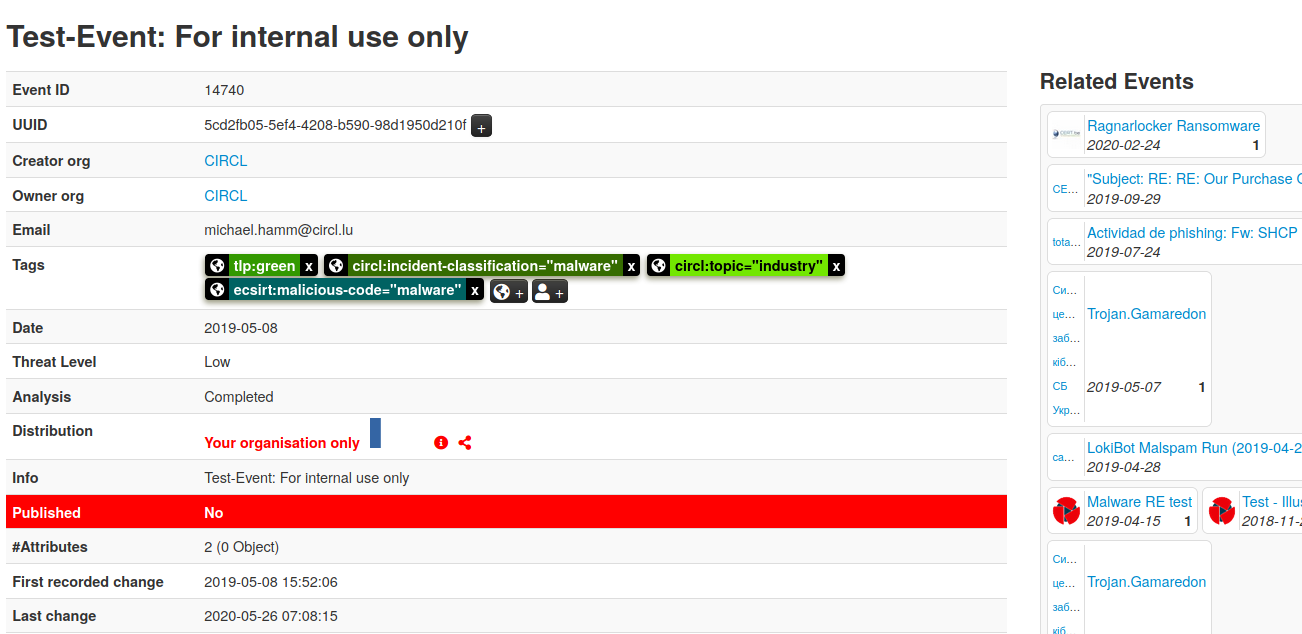
\includegraphics[scale=0.25]{images/misp_1.png}
        \captionsetup{labelformat=empty,labelsep=none}
        \transparent{0.7}%
        \caption[]{\tiny Event Overview: https://misppriv.circl.lu/}
    \end{figure}
\end{frame}


\begin{frame}[fragile]
  \frametitle{4.3 Enrich Online}
    \begin{figure}
        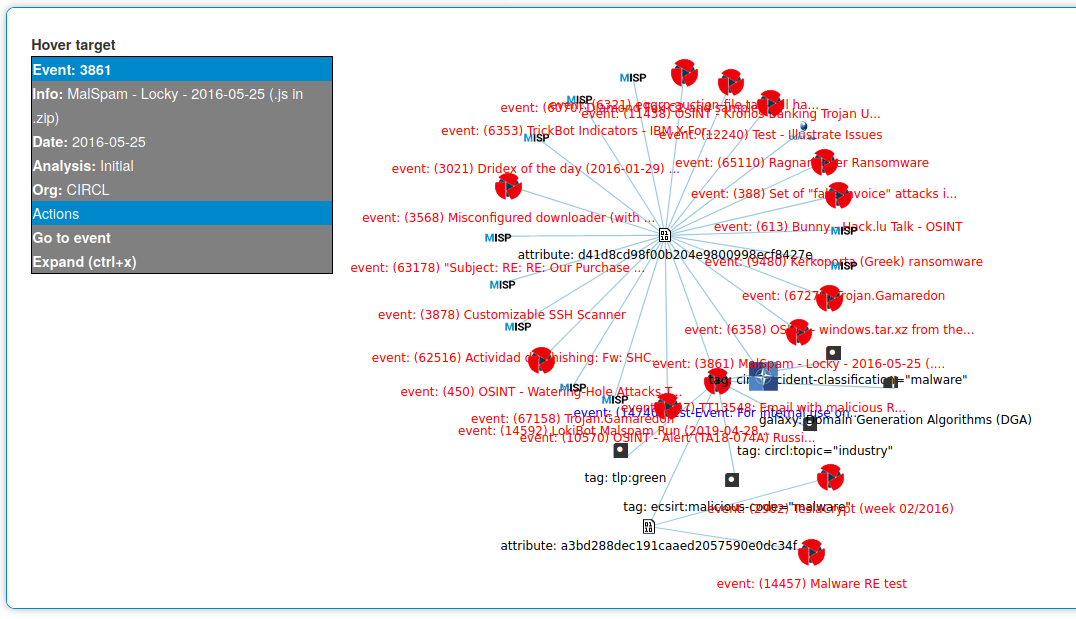
\includegraphics[scale=0.27]{images/misp_2.png}
        \captionsetup{labelformat=empty,labelsep=none}
        \transparent{0.7}%
        \caption[]{\tiny Correlation Graph: https://misppriv.circl.lu/}
    \end{figure}
\end{frame}


\begin{frame}[fragile]
  \frametitle{4.4 Static Analysis}
    \begin{itemize}
        \item Perfect disassembly $\to$ Unsolved problem
        \item Linear disassembly
        \begin{itemize}
            \item Identify the program code
            \item Decode the bytes
        \end{itemize}
        \item Linear disassembly limitations
        \begin{itemize}
            \item Don't know how instructions get decoded by CPU
            \item Could not counter fight obfuscation
        \end{itemize}
        \item Obfuscation techniques
        \begin{itemize}
            \item Packing
            \item Resource Obfuscation
            \item Anti-Disassembly
            \item Dynamic Data Download
        \end{itemize}
        \item Counter fight obfuscation
        \begin{itemize}
            \item Dynamic Analysis
            \item Run malware in isolated environment
        \end{itemize}
    \end{itemize}
\end{frame}


\begin{frame}[fragile]
  \frametitle{4.5 x86 Assembly: General-Purpose Registers}
    \begin{figure}
        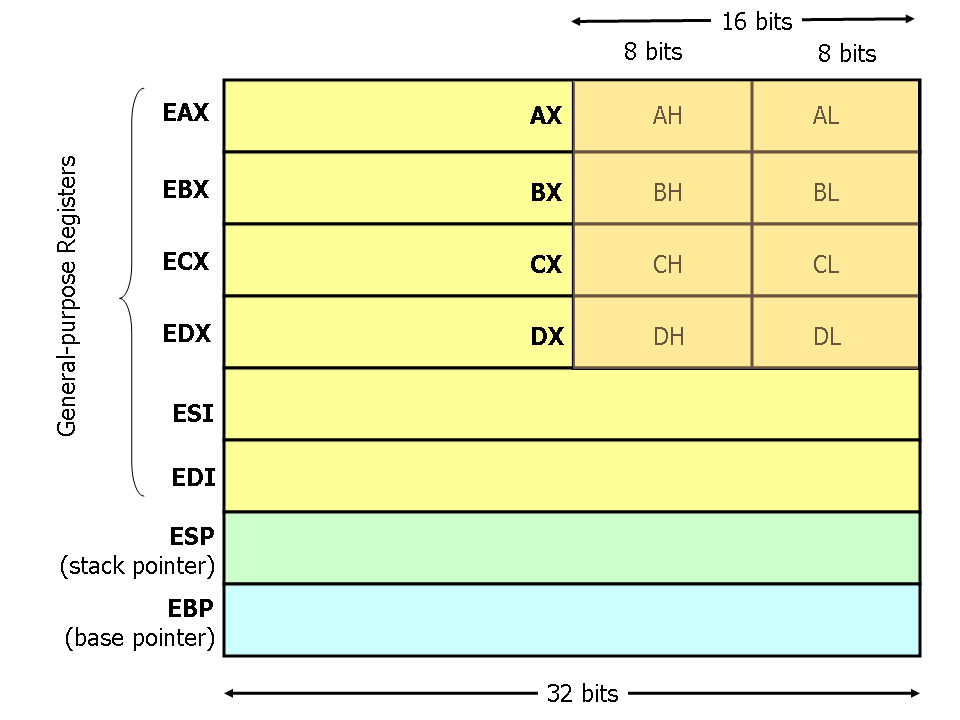
\includegraphics[scale=0.34]{images/x86-registers.png}
        \captionsetup{labelformat=empty,labelsep=none}
        \transparent{0.7}%
        \caption[]{\tiny https://www.cs.virginia.edu/~evans/cs216/guides/x86.html}
    \end{figure}
\end{frame}


\begin{frame}[fragile]
  \frametitle{4.5 x86 Assembly: Stack and Control Flow Registers}
    \begin{figure}
        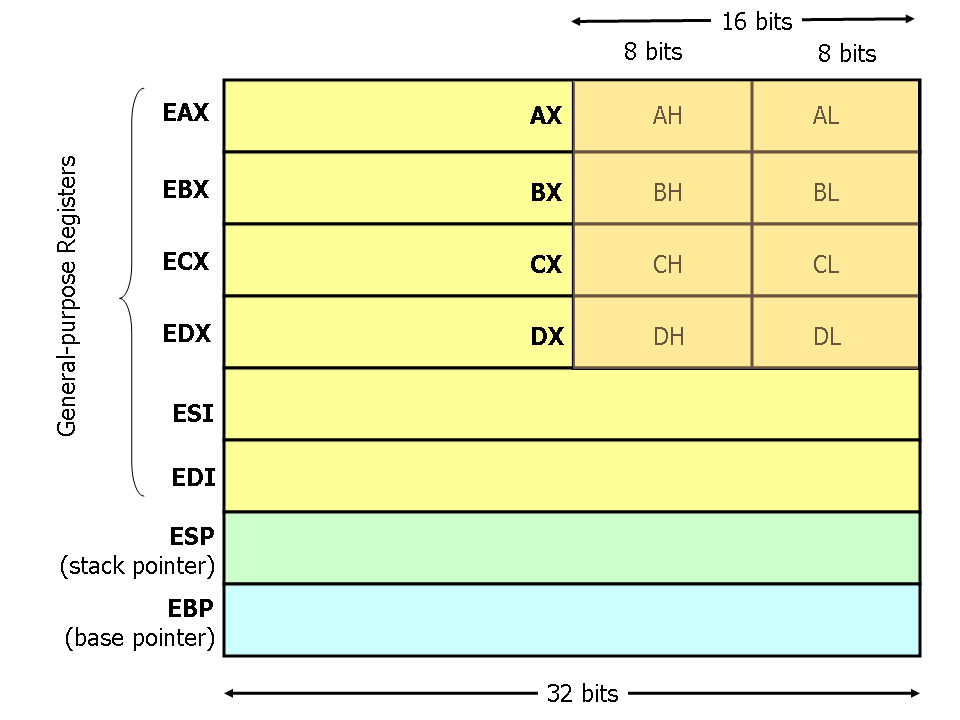
\includegraphics[scale=0.34]{images/x86-registers.png}
        \captionsetup{labelformat=empty,labelsep=none}
        \transparent{0.7}%
        \caption[]{\tiny https://www.cs.virginia.edu/~evans/cs216/guides/x86.html}
    \end{figure}
\end{frame}


\begin{frame}[fragile]
  \frametitle{4.5 x86 Assembly: Instructions}
  \begin{lstlisting}[basicstyle=\tiny]
Arithmetic:      add ebx, 100       Adds 100 to the value in EBX
                 sub ecx, 123       Substract 123 from the value in ECX
	         inc ah             Increments value in AH by 1
	         dec al             Decrements value in AL by 1

Data Movement:   mov eax, ebx       Move value in EBX into register EAX
                 mov eax, [0x4711]  Move value at memory 0x4711 intp EAX
		 mov eax, 1         Move the value 1 into register EAX
		 mov [0x4711], eax  Move value of EAX into memory 0x4711

Stack:           push 1             Increment ESP; Store 1 on top of stack
                 pop eax            Store highest value in EAX; Decrement ESP

Control Flow:    call [address]     1. Put EIP on top of the stack
                                    2. Put [address] into EIP
                 ret                1. Popped top of teh stack into EIP
		                    2. Resume execution
		 jmp 0x1234         Start executing progamm code at 0x1234
		 cmp eax, 100       1. Compares value in EAX with 100
		                    2. Based on result set EFLAGS register
		 jge 0x1234         1. Interpret EFLAGS register
		                    2. If 'greater' or 'equal' flag then jump
  \end{lstlisting}
\end{frame}


\begin{frame}[fragile]
  \frametitle{4.5 x86 Assembly: Control Flow Graphs}
  \begin{lstlisting}[basicstyle=\tiny]
start:             Symbol for address of next instruction
mov eax, 3         Initialize a counter of 3 into EAX

loop:              Symbol for address of next instruction
sub eax, 1         Substract 1 from value in EAX
cmp 0, eax         Compare value in EAX with 0; Set EFLAGS
jne $loop          IF EFLAGS 'not equal' jump to 'loop'

end:               Symbol for address of next instruction
mov eax, 12











.
  \end{lstlisting}
\end{frame}


\begin{frame}[fragile]
  \frametitle{4.5 x86 Assembly: Control Flow Graphs}
  \begin{lstlisting}[basicstyle=\tiny]
start:             Symbol for address of next instruction
mov eax, 3         Initialize a counter of 3 into EAX

loop:              Symbol for address of next instruction
sub eax, 1         Substract 1 from value in EAX
cmp 0, eax         Compare value in EAX with 0; Set EFLAGS
jne $loop          IF EFLAGS 'not equal' jump to 'loop'

end:               Symbol for address of next instruction
mov eax, 12


      -------------    ------>    -------------    ------>    ------------- 
     | start:      |      --->   | loop:       |             | end:        |
     | ----------- |     |       | ----------- |             | ----------- |
     |             |     |       |             |             |             |
     | mov eax, 3  |     |       | sub eax, 1  |             | mov eax, 12 |
     |             |     |       | cmp 0, eax  |             |             |
      -------------       ----   | jne $loop   |              -------------
			         |             | 
			          ------------- 
.
  \end{lstlisting}
\end{frame}


\begin{frame}[fragile]
  \frametitle{4.6 Dynamic Analysis}
    \begin{figure}
        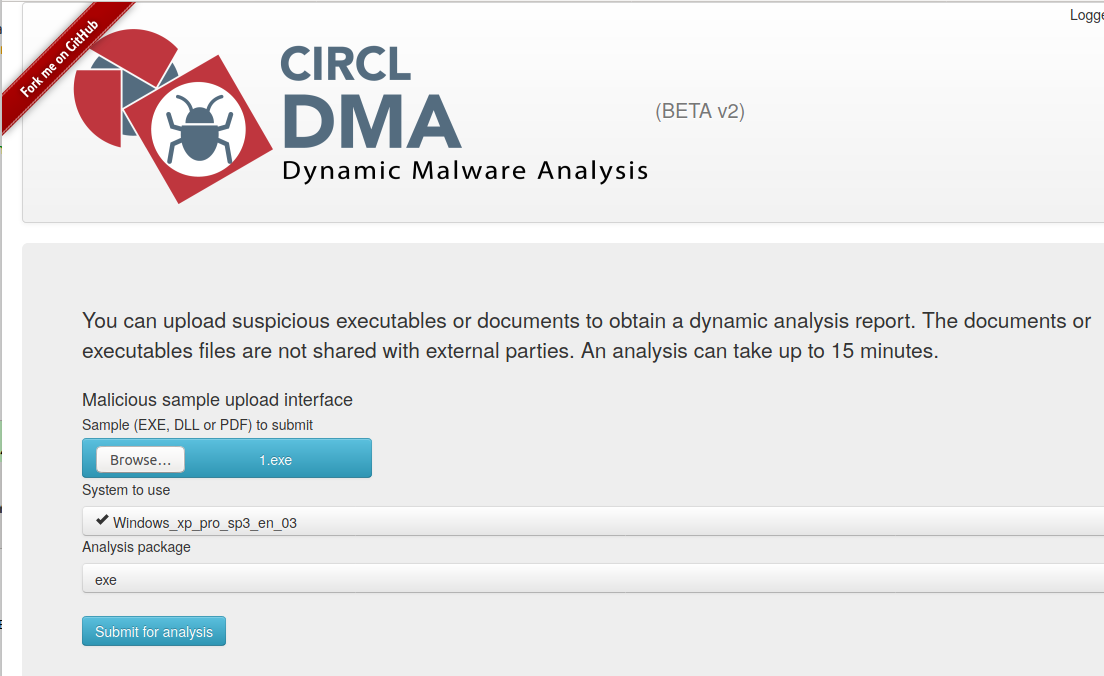
\includegraphics[scale=0.27]{images/dma_1.png}
        \captionsetup{labelformat=empty,labelsep=none}
        \transparent{0.7}%
        \caption[]{\tiny Upload a 1.exe: https://circl.lu/services/dynamic-malware-analysis/}
    \end{figure}
\end{frame}


\begin{frame}[fragile]
  \frametitle{4.6 Dynamic Analysis}
    \begin{figure}
        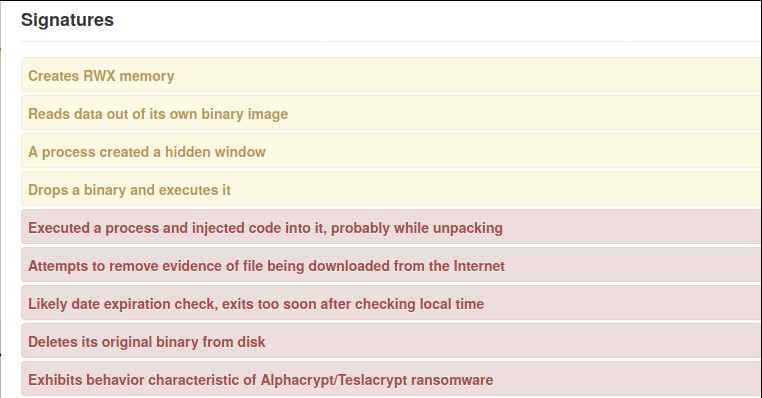
\includegraphics[scale=0.4]{images/dma_2a.png}
        \captionsetup{labelformat=empty,labelsep=none}
        \transparent{0.7}%
        \caption[]{\tiny Signatures and Screenshots: https://circl.lu/services/dynamic-malware-analysis/}
    \end{figure}
\end{frame}


\begin{frame}[fragile]
  \frametitle{4.6 Dynamic Analysis}
    \begin{figure}
        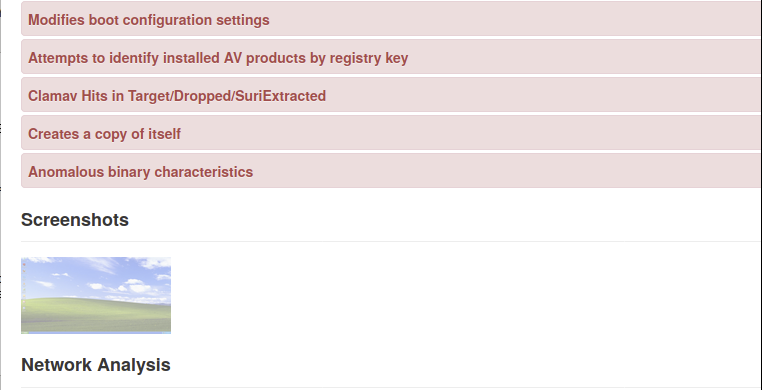
\includegraphics[scale=0.4]{images/dma_2b.png}
        \captionsetup{labelformat=empty,labelsep=none}
        \transparent{0.7}%
        \caption[]{\tiny Signatures and Screenshots: https://circl.lu/services/dynamic-malware-analysis/}
    \end{figure}
\end{frame}


\begin{frame}[fragile]
  \frametitle{4.6 Dynamic Analysis}
    \begin{figure}
        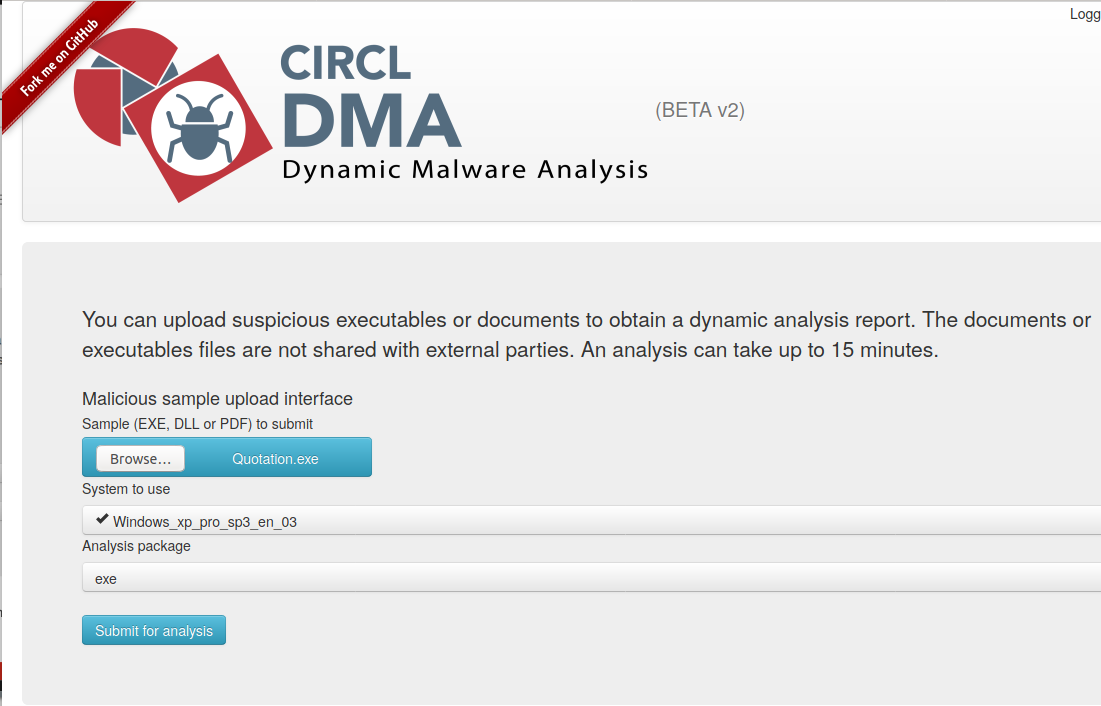
\includegraphics[scale=0.26]{images/dma_3.png}
        \captionsetup{labelformat=empty,labelsep=none}
        \transparent{0.7}%
        \caption[]{\tiny Upload a Quotation.exe: https://circl.lu/services/dynamic-malware-analysis/}
    \end{figure}
\end{frame}


\begin{frame}[fragile]
  \frametitle{4.6 Dynamic Analysis}
    \begin{figure}
        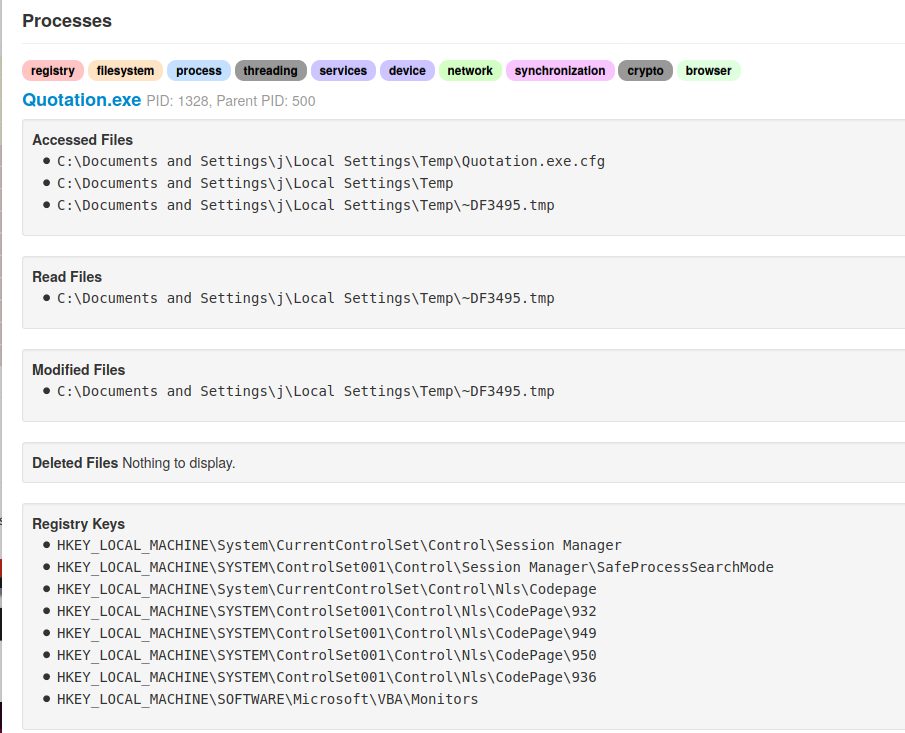
\includegraphics[scale=0.25]{images/dma_4.png}
        \captionsetup{labelformat=empty,labelsep=none}
        \transparent{0.7}%
        \caption[]{\tiny Access to Files and Registry: https://circl.lu/services/dynamic-malware-analysis/}
    \end{figure}
\end{frame}











%
% This work is licensed under a Creative Commons Attribution-ShareAlike 4.0 International License.
% http://creativecommons.org/licenses/by-sa/4.0/
%

% DO NOT COMPILE THIS FILE DIRECTLY!
% This is included by the other .tex files.


\begin{frame}
    
\includegraphics[scale=0.3]{images/logo-circl-Forensics.png}
    \begin{itemize}
        \item[]
        \item[]
        \item[] 5. Analysing files
    \end{itemize}
\end{frame}


\begin{frame}[fragile]
  \frametitle{5.1 Analysing files}
    \begin{itemize}
       \item Standard Linux commands
            \begin{itemize}
                \item[] \texttt{file}
                \item[] \texttt{strings}
                \item[] \texttt{exiftool}
                \item[] \texttt{md5sum, sha1sum}
                \item[] \texttt{7z}
                \item[] .....
            \end{itemize}
       \item Dedicated tools
            \begin{itemize}
                \item[] \texttt{oledump.py}
                \item[] \texttt{pdfid.py, pdf-parser.py}
                \item[] \texttt{VirusTotal tools}
                \item[] .....
            \end{itemize}
       \item Exercise: Run \texttt{exiftool} on carving recovered documents
    \end{itemize}
\end{frame}


\begin{frame}[fragile]
  \frametitle{5.2 Analysing files}
    \begin{itemize}
       \item Online resources
            \begin{itemize}
                \item[] \href{https://www.nist.gov/software-quality-group/national-software-reference-library-nsrl}{NSRL - National Software Reference Library}
                \item[] \href{https://www.virustotal.com/}{VirusTotal}
                \item[] \href{https://www.circl.lu/services/dynamic-malware-analysis/}{CIRCL: DMA}
                \item[] \href{https://www.circl.lu/services/misp-malware-information-sharing-platform/}{CIRCL: MISP Threat Sharing Platform}
                \item[]
            \end{itemize}
       \item Demo: Search MD5
            \begin{itemize}
                \item[] \texttt{A479C4E7ED87AEDAFAD7D9936DC80115}
                \item[] \texttt{81e9036aed5502446654c8e5a1770935}
                \item[] 
            \end{itemize}
       \item Analysing files could become a training on it's own
    \end{itemize}
\end{frame}





%
% This work is licensed under a Creative Commons Attribution-ShareAlike 4.0 International License.
% http://creativecommons.org/licenses/by-sa/4.0/
%

% DO NOT COMPILE THIS FILE DIRECTLY!
% This is included by the other .tex files.


\begin{frame}
    
\includegraphics[scale=.3]{images/logo-circl-Forensics.png}
    \begin{itemize}
        \item[]
        \item[]
        \item[] 6. Live Response
    \end{itemize}
\end{frame}


\begin{frame}
  \frametitle{6.1 Volatile Data}
  \begin{itemize}
      \item Memory dump
      \item Live analysis:
      \begin{itemize}
          \item[] $\to$ System time
          \item[] $\to$ Logged-on users
          \item[] $\to$ Open files
          \item[] $\to$ Network -connections -status
          \item[] $\to$ Process information -memory
          \item[] $\to$ Process / port mapping
          \item[] $\to$ Clipboard content
          \item[] $\to$ Services
          \item[] $\to$ Command history
          \item[] $\to$ Mapped drives / shares
          \item[] $\to$ !!! Do not store information on the subject system !!!
      \end{itemize}
      \item Image of live system $($Possible issues$)$
      \item Shutdown and image if possible
  \end{itemize}
\end{frame}


\begin{frame}[fragile]
  \frametitle{6.1 Collecting Volatile Data}
  \begin{lstlisting}[basicstyle=\tiny]
  https://docs.microsoft.com/en-us/sysinternals/
  ----------------------------------------------
  \end{lstlisting}
  \begin{itemize}
        \item System Time
\begin{lstlisting}[basicstyle=\tiny]
> date /t & time /t            # Don't foget to note wall-clock-time
    Tue 03/26/2019             # Note timezone of PC
    01:31 PM
\end{lstlisting}
        \item Loggedon Users
\begin{lstlisting}[basicstyle=\tiny]
> net session

> .\PsLoggedon.exe
    Users logged on locally:
         3/26/2019 1:30:23 PM       John-PC\John
    No one is logged on via resource shares.

> .\logonsessions.exe
    [5] Logon session 00000000:0001ad9d:
        User name:    John-PC\John
        Auth package: NTLM
        Logon type:   Interactive
        Session:      1
        Sid:          S-1-5-21-3031575581-801213887-4188682232-1001
        Logon time:   3/26/2019 1:30:23 PM
        Logon server: JOHN-PC
\end{lstlisting}
    \end{itemize}
\end{frame}


\begin{frame}[fragile]
  \frametitle{6.1 Collecting Volatile Data}
  \begin{itemize}
        \item Open Files
\begin{lstlisting}[basicstyle=\tiny]
> net file

> .\psfile.exe
\end{lstlisting}
        \item Network Connections and Status
\begin{lstlisting}[basicstyle=\tiny]
> netstat -anob
    Proto  Local Address      Foreign Address     State         PID    RpcSs
    TCP    0.0.0.0:135        0.0.0.0:0           LISTENING     696    [svchost.exe]
    TCP    0.0.0.0:445        0.0.0.0:0           LISTENING     4
    TCP    0.0.0.0:554        0.0.0.0:0           LISTENING     2504   [wmpnetwk.exe]
    TCP    0.0.0.0:10243      0.0.0.0:0           LISTENING     4
    TCP    0.0.0.0:49152      0.0.0.0:0           LISTENING     364    [wininit.exe]

> netstat -rn
    Network Destination        Netmask          Gateway       Interface  Metric
              0.0.0.0          0.0.0.0         10.0.2.2        10.0.2.15     10
             10.0.2.0    255.255.255.0         On-link         10.0.2.15    266
            10.0.2.15  255.255.255.255         On-link         10.0.2.15    266

> ipconfig /all
\end{lstlisting}
    \end{itemize}
\end{frame}


\begin{frame}[fragile]
  \frametitle{6.1 Collecting Volatile Data}
  \begin{itemize}
        \item Running Processes
\begin{lstlisting}[basicstyle=\tiny]
> tasklist
    Image Name                     PID Session Name        Session#    Mem Usage
    ========================= ======== ================ =========== ============
    System                           4 Services                   0        600 K
    smss.exe                       252 Services                   0        792 K
    csrss.exe                      328 Services                   0      3,224 K
    wininit.exe                    364 Services                   0      3,316 K
    csrss.exe                      372 Console                    1      4,196 K
    winlogon.exe                   400 Console                    1      6,272 K
    services.exe                   460 Services                   0      6,628 K
    lsass.exe                      468 Services                   0      8,428 K
    lsm.exe                        476 Services                   0      3,040 K
    svchost.exe                    584 Services                   0      6,596 K
    cmd.exe                       3100 Console                    1      2,480 K

> tasklist /svc
    Image Name                     PID Services
    ========================= ======== ============================================
    svchost.exe                    584 DcomLaunch, PlugPlay, Power
    svchost.exe                    696 RpcEptMapper, RpcSs
    svchost.exe                    792 Audiosrv, Dhcp, eventlog,
                                       HomeGroupProvider, lmhosts, wscsvc
    svchost.exe                    844 AudioEndpointBuilder, CscService,
                                       HomeGroupListener, Netman, TrkWks, UxSms,
    svchost.exe                    876 EventSystem, fdPHost, FontCache, netprofm,
                                       nsi, WdiServiceHost
\end{lstlisting}
    \end{itemize}
\end{frame}


\begin{frame}[fragile]
  \frametitle{6.1 Collecting Volatile Data}
  \begin{itemize}
        \item Running Processes
\begin{lstlisting}[basicstyle=\tiny]
> .\pslist.exe -x

> .\pslist.exe -t
    Name                             Pid Pri Thd  Hnd      VM      WS    Priv
    explorer                        1252   8  26  912  212044   47672   36304
      VBoxTray                       360   8  12  153   61384    5624    1476
      cmd                            548   8   1   24   29256    2564    2628
        pslist                      3452  13   1  123   45908    3640    1652
      WzPreloader                   1244   8   6  119  109748    9064   11224
      cmd                           3100   8   1   20   27464    2480    1804

> .\Listdlls.exe

> .\handle.exe
\end{lstlisting}
        \item Processes/Port Mapping
\begin{lstlisting}[basicstyle=\tiny]
> .\tcpvcon -n -c -a
    TCP,svchost.exe,692,LISTENING,0.0.0.0,0.0.0.0
    TCP,System,4,LISTENING,10.0.2.15,0.0.0.0
    TCP,wmpnetwk.exe,2428,LISTENING,0.0.0.0,0.0.0.0
    TCP,wininit.exe,364,LISTENING,0.0.0.0,0.0.0.0
    TCP,svchost.exe,776,LISTENING,0.0.0.0,0.0.0.0
    TCP,svchost.exe,896,LISTENING,0.0.0.0,0.0.0.0
    TCP,services.exe,460,LISTENING,0.0.0.0,0.0.0.0
\end{lstlisting}
    \end{itemize}
\end{frame}


\begin{frame}[fragile]
  \frametitle{6.1 Collecting Volatile Data}
  \begin{itemize}
        \item Command History
\begin{lstlisting}[basicstyle=\tiny]
> doskey /history
    netstat -anob
    .\Listdlls.exe
    .\handle.exe
    .\tcpvcon -n -c -a
    cls
    doskey /history
\end{lstlisting}
        \item Processes/Port Mapping
\begin{lstlisting}[basicstyle=\tiny]

\end{lstlisting}
    \end{itemize}
\end{frame}


\begin{frame}[fragile]
  \frametitle{6.2 Non Volatile Data}
  \begin{itemize}
        \item Clear Pagefile at shutdown
\begin{lstlisting}[basicstyle=\tiny]
> reg QUERY "HKLM\SYSTEM\CurrentControlSet\Control\Session Manager\Memory Management"
    .....
    ClearPageFileAtShutdown    REG_DWORD    0x0
    .....
\end{lstlisting}
        \item Update Last Access disabled
\begin{lstlisting}[basicstyle=\tiny]
> reg QUERY "HKLM\SYSTEM\CurrentControlSet\Control\FileSystem"
    .....
    NtfsDisableLastAccessUpdate    REG_DWORD    0x0
    .....
\end{lstlisting}
        \item Autostart locations
\begin{lstlisting}[basicstyle=\tiny]
> .\Autoruns.exe
\end{lstlisting}
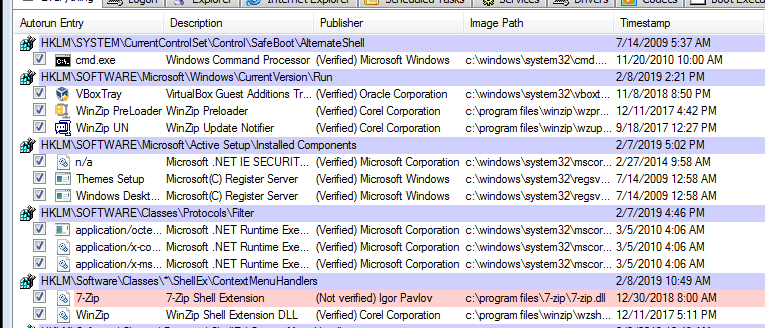
\includegraphics[scale=.27]{images/f11_autorun.png}
  \end{itemize}
\end{frame}


\begin{frame}[fragile]
  \frametitle{6.3 Across the network}
  \begin{itemize}
        \item Get Nmap command-line zipfile
	\item[] \url{https://nmap.org/download.html}
	\item[]
        \item On Linux set up a netcat listener
\begin{lstlisting}[basicstyle=\tiny]
nc -k -l 9999 >> logfile.txt
\end{lstlisting}
        \item Sending from subject system
\begin{lstlisting}[basicstyle=\tiny]
ncat aaa.bbb.ccc.ddd 9999

echo "Date and Time" | ncat.exe aaa.bbb.ccc.ddd 9999
date /t | ncat.exe aaa.bbb.ccc.ddd 9999
time /t | ncat.exe aaa.bbb.ccc.ddd 9999
echo "-------------" | ncat.exe aaa.bbb.ccc.ddd 9999
\end{lstlisting}
  \end{itemize}
\end{frame}








%
% This work is licensed under a Creative Commons Attribution-ShareAlike 4.0 International License.
% http://creativecommons.org/licenses/by-sa/4.0/
%

% DO NOT COMPILE THIS FILE DIRECTLY!
% This is included by the other .tex files.


\begin{frame}
    
\includegraphics[scale=0.3]{images/logo-circl-Forensics.png}
    \begin{itemize}
        \item[]
        \item[]
        \item[] 7. Memory Forensics
    \end{itemize}
\end{frame}


\begin{frame}
  \frametitle{7.1 About Memory Forensics}
    \begin{itemize}
        \item Information expected
            \begin{itemize}
                \item Network connections
		\item Processes (hidden)
		\item Services (listening)
                \item Malware
                \item Registry content
                \item DLL analysis
                \item Passwords in clear text
            \end{itemize}
        \item History
            \begin{itemize}
                \item 2005: String search
		\item $\to$ EProcess structures
            \end{itemize}
        \item Finding EProcess structures
            \begin{itemize}
		\item Find the doubly linked list (ntoskrnl.exe)
		\item Brute Force searching
            \end{itemize}
    \end{itemize}
\end{frame}


\begin{frame}
  \frametitle{7.2 Get your memory dump}
    \begin{itemize}
        \item Page file, swap area: \texttt{pagefile.sys}
        \item Memory dump
            \begin{itemize}
		    \item[] \url{http://www.msuiche.net}
		    \item[] \texttt{DumpIt.exe}
                    \item[] 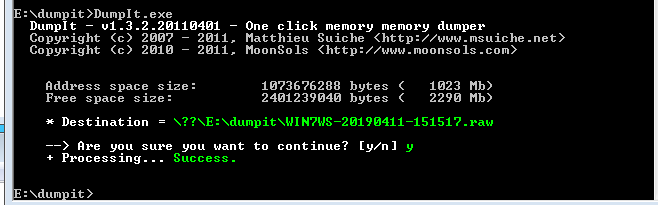
\includegraphics[scale=0.5]{images/f12_dumpit.png}
		    \item[] 
            \end{itemize}
        \item Hibernation file: \texttt{hiberfil.sys}
            \begin{itemize}
		    \item[] \texttt{powercfg /h[ibernate] [on|off]}
		    \item[] \texttt{psshutdown -h}
            \end{itemize}
    \end{itemize}
\end{frame}


\begin{frame}
  \frametitle{7.2 DumpIt}
  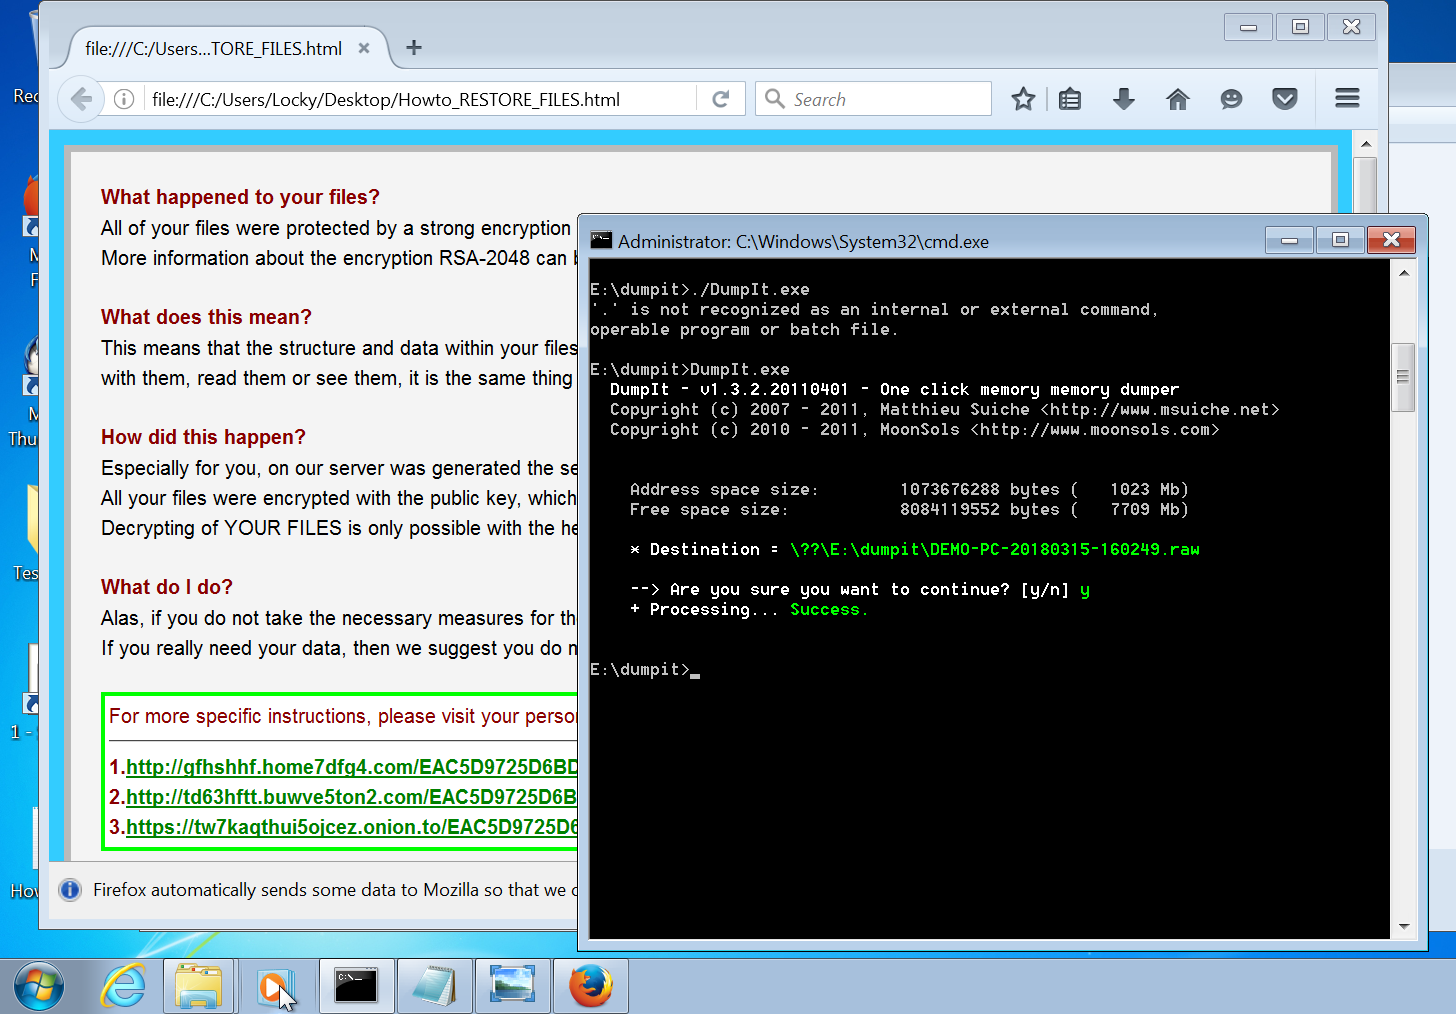
\includegraphics[scale=0.2]{images/f11_memdump.png}
\end{frame}

\begin{frame}
  \frametitle{7.3 Mandiant Redline - Malware Risk Index}
  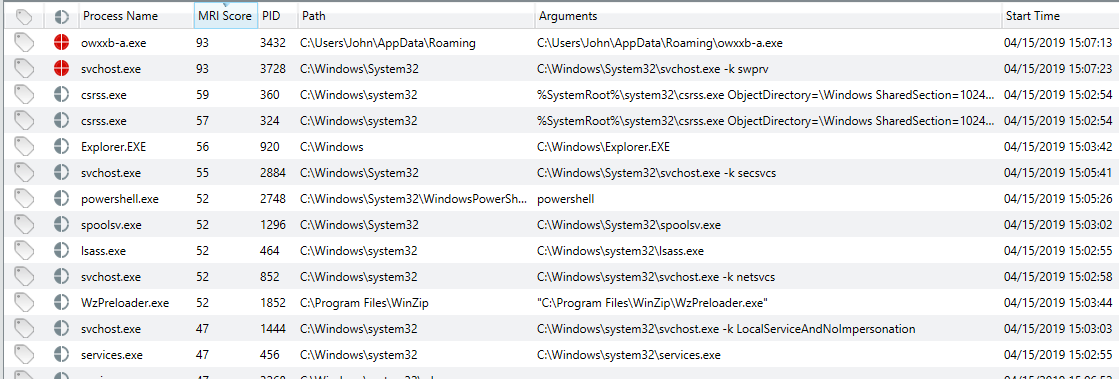
\includegraphics[scale=0.38]{images/f12_redline-1.png}
\end{frame}

\begin{frame}
  \frametitle{7.3 Mandiant Redline - Malware Risk Index}
  \begin{figure}
    \begin{center}
      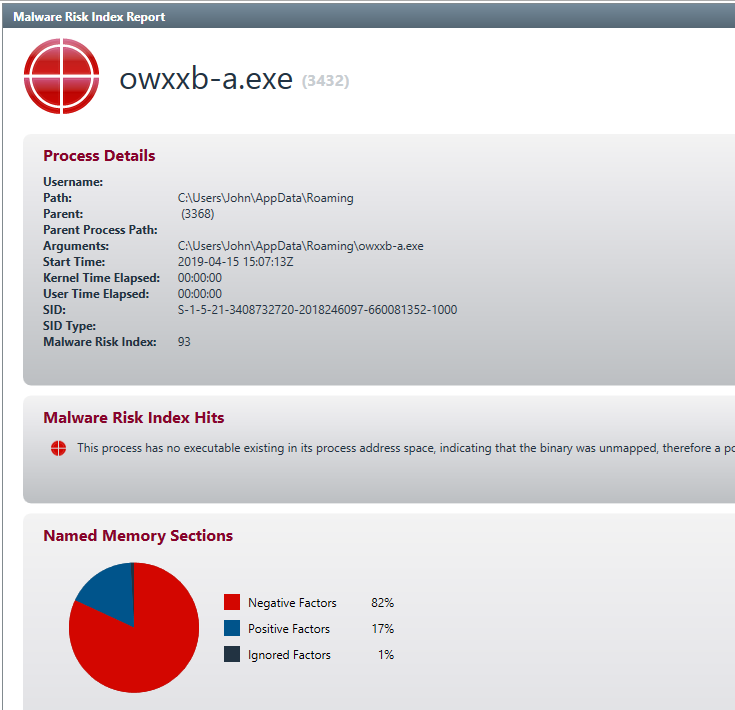
\includegraphics[scale=0.28]{images/f12_redline-2.png}

      \vspace{0.2cm}

      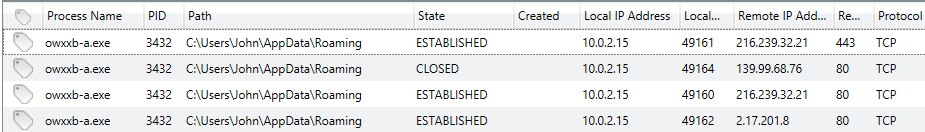
\includegraphics[scale=0.35]{images/f12_redline-3.png}
    \end{center}
  \end{figure}
\end{frame}

\begin{frame}
  \frametitle{7.3 Mandiant Redline - Malware Risk Index}
  \begin{figure}
    \begin{center}
      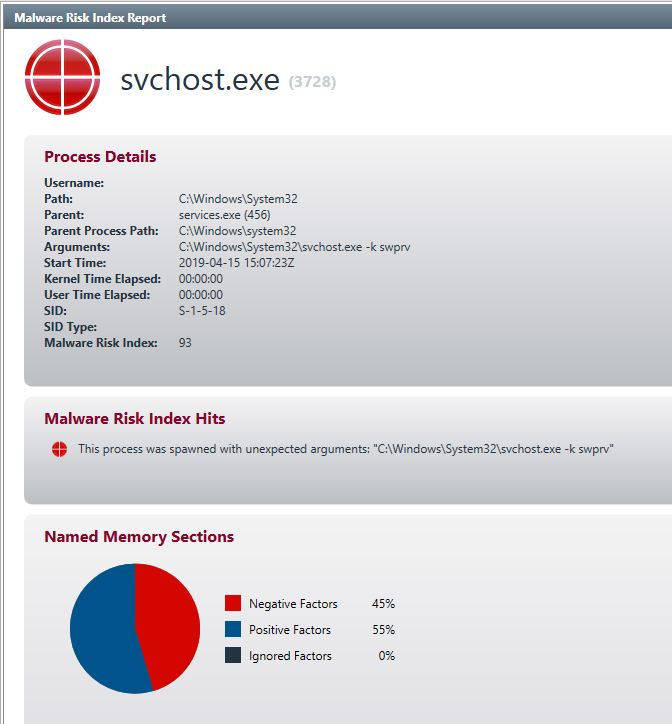
\includegraphics[scale=0.35]{images/f12_redline-4.png}
    \end{center}
  \end{figure}
\end{frame}

\begin{frame}
  \frametitle{7.3 Mandiant Redline - Hierarchical}
  \begin{figure}
    \begin{center}
      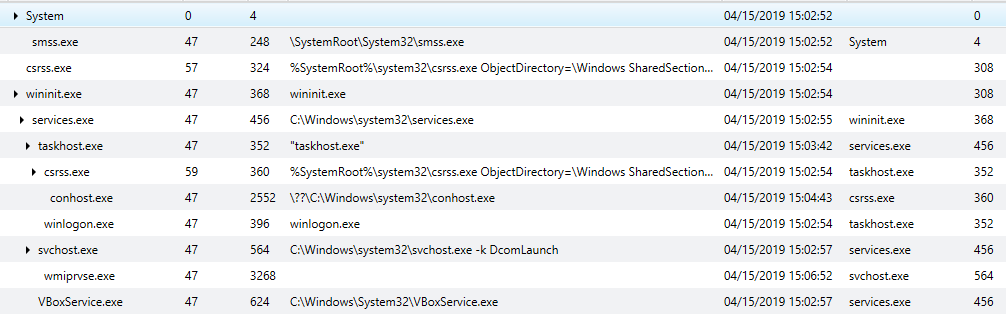
\includegraphics[scale=0.42]{images/f12_redline-5.png}

      \vspace{0.2cm}

      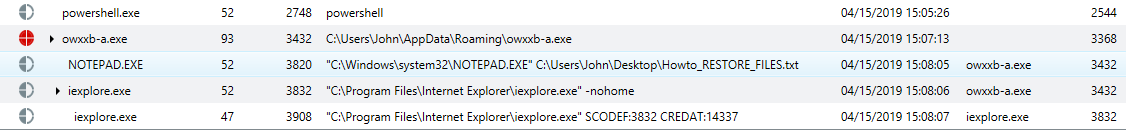
\includegraphics[scale=0.4]{images/f12_redline-7.png}
    \end{center}
  \end{figure}
\end{frame}

\begin{frame}
  \frametitle{7.3 Mandiant Redline - Timeline}
  \begin{figure}
    \begin{center}
      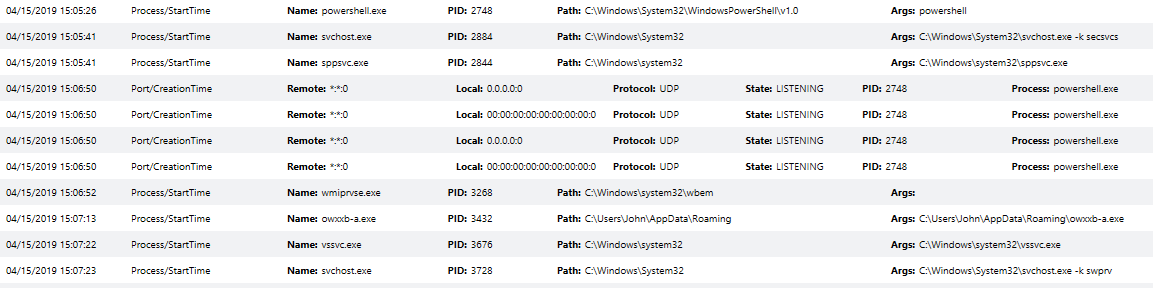
\includegraphics[scale=0.37]{images/f12_redline-6.png}

      \vspace{0.2cm}

      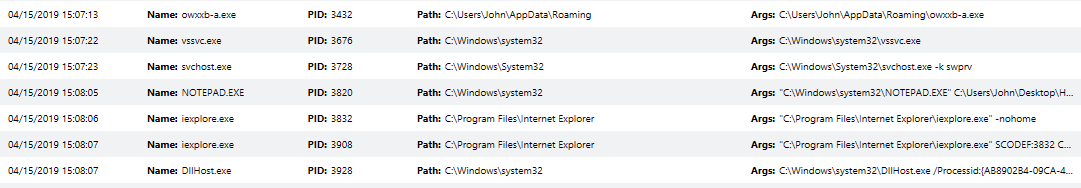
\includegraphics[scale=0.4]{images/f12_redline-8.png}
    \end{center}
  \end{figure}
\end{frame}


\begin{frame}[fragile]
  \frametitle{7.4 Volatility: Overview}
    \begin{itemize}
        \item[]
            \begin{itemize}
                \item[] \texttt{volatility --info}
                \item[] \texttt{volatility -h}
                \begin{lstlisting}[basicstyle=\tiny]
...
imagecopy      	Copies a physical address space out as a raw DD image
imageinfo      	Identify information for the image
...
pslist         	Print all running processes by following the EPROCESS lists 
psscan         	Scan Physical memory for _EPROCESS pool allocations
pstree         	Print process list as a tree
psxview        	Find hidden processes with various process listings
...
sockets        	Print list of open sockets
sockscan       	Scan Physical memory for _ADDRESS_OBJECT objects (tcp sockets)
...
                \end{lstlisting}
                \item[] \texttt{volatility -f [filename] [plugin] [options]}
                \item[]
                \item[] \texttt{volatility -f memdump.raw imageinfo}
                \item[]
            \end{itemize}
    \end{itemize}
\end{frame}


\begin{frame}[fragile]
  \frametitle{7.4 Volatility: Overview}
    \begin{itemize}
        \item[]
            \begin{itemize}
                \item[] \texttt{volatility -f memdump.raw imageinfo}
                \item[]
                \begin{lstlisting}[basicstyle=\tiny]
Volatility Foundation Volatility Framework 2.6
INFO    : volatility.debug    : Determining profile based on KDBG search...

          Suggested Profile(s) : Win7SP1x86_23418, Win7SP0x86, Win7SP1x86
                     AS Layer1 : IA32PagedMemory (Kernel AS)
                     AS Layer2 : FileAddressSpace
                      PAE type : No PAE
                           DTB : 0x185000L
                          KDBG : 0x82968c28L
          Number of Processors : 1
     Image Type (Service Pack) : 1
                KPCR for CPU 0 : 0x82969c00L
             KUSER_SHARED_DATA : 0xffdf0000L
           Image date and time : 2019-04-15 15:08:11 UTC+0000
     Image local date and time : 2019-04-15 17:08:11 +0200
		\end{lstlisting}
                \item[]
                \item[] \texttt{volatility -f memdump.raw kdbgscan}
		\item[] \texttt{volatility --profile=Win7SP1x86 -f [filename] [plugin]}
		\item[] \texttt{export VOLATILITY\_PROFILE=Win7SP1x86}
            \end{itemize}
    \end{itemize}
\end{frame}


\begin{frame}[fragile]
  \frametitle{7.5 Volatility: Process Analysis}
    \begin{itemize}
        \item[] \texttt{pslist}
            \begin{itemize}
                \item Running processes
                \item Process IP - PID
                \item Parent PIP - PPID
                \item Start time
            \end{itemize}
        \item[] \texttt{pstree}
            \begin{itemize}
                \item Like \texttt{pslist}
                \item Visual child-parent relation
            \end{itemize}
        \item[] \texttt{psscan}
            \begin{itemize}
                \item Brute Force
                \item Find inactive and/or hidden processes
            \end{itemize}
        \item[] \texttt{psxview}
            \begin{itemize}
                \item Run and compare some tests
                \item Correlate \texttt{psscan} and \texttt{pslist}
            \end{itemize}
    \end{itemize}
\end{frame}


\begin{frame}[fragile]
  \frametitle{7.5 Volatility: Process Analysis}
    \texttt{\footnotesize volatility --profile=Win7SP1x86 -f Win-Enc-20190415.raw pslist}
    \begin{lstlisting}[basicstyle=\tiny]
Offset(V)  Name             PID   PPID Thds  Hnds Ses Wow64 Start          
---------- ------------- ------ ------ ---- ----- --- -------------------------
0x84233af0 System             4      0   70   505 ---    0 2019-04-15 15:02:52 UTC+0000 
0x848d8288 smss.exe         248      4    2    29 ---    0 2019-04-15 15:02:52 UTC+0000
0x8487a700 csrss.exe        324    308    9   384   0    0 2019-04-15 15:02:54 UTC+0000
0x84fbb530 csrss.exe        360    352    7   274   1    0 2019-04-15 15:02:54 UTC+0000
0x84fc3530 wininit.exe      368    308    3    77   0    0 2019-04-15 15:02:54 UTC+0000
0x84fd0530 winlogon.exe     396    352    4   112   1    0 2019-04-15 15:02:54 UTC+0000
0x85048a18 services.exe     456    368    8   203   0    0 2019-04-15 15:02:55 UTC+0000
0x8505ac00 lsass.exe        464    368    7   580   0    0 2019-04-15 15:02:55 UTC+0000
0x8505caa0 lsm.exe          472    368   10   145   0    0 2019-04-15 15:02:55 UTC+0000
...
...
...
0x85050b60 WmiPrvSE.exe    3268    564    9   175   0    0 2019-04-15 15:06:52 UTC+0000
0x8438bd40 owxxb-a.exe     3432   3368   15   471   1    0 2019-04-15 15:07:13 UTC+0000
0x84394030 VSSVC.exe       3676    456    6   123   0    0 2019-04-15 15:07:22 UTC+0000
0x84394488 svchost.exe     3728    456    6    70   0    0 2019-04-15 15:07:23 UTC+0000
0x84a243c8 notepad.exe     3820   3432    1    64   1    0 2019-04-15 15:08:05 UTC+0000
0x846d8030 iexplore.exe    3832   3432   19   427   1    0 2019-04-15 15:08:06 UTC+0000
0x846d2d40 iexplore.exe    3908   3832   11   293   1    0 2019-04-15 15:08:07 UTC+0000
0x846e5a58 dllhost.exe     3928    564    6    94   1    0 2019-04-15 15:08:07 UTC+0000
0x84684d40 dllhost.exe     4012    564   10   212   1    0 2019-04-15 15:08:08 UTC+0000
    \end{lstlisting}
\end{frame}


\begin{frame}[fragile]
  \frametitle{7.5 Volatility: Process Analysis}
    \texttt{\footnotesize volatility --profile=Win7SP1x86 -f Win-Enc-20190415.raw pslist}
    \begin{lstlisting}[basicstyle=\tiny]
Offset(P)  Name          PID pslist psscan thrdproc pspcid csrss session deskthrd
---------- ---------- ------ ------ ------ -------- ------ ----- ------- --------
.....
.....
0x3f60f030 taskhost.exe     352 True   True   True     True   True  True    True
0x3fa84d40 dllhost.exe     4012 True   True   True     True   True  True    True
0x3ec23148 spoolsv.exe     1296 True   True   True     True   True  True    True
0x3f63f470 explorer.exe     920 True   True   True     True   True  True    True
0x3ff0bd40 owxxb-a.exe     3432 True   True   True     True   True  True    True
0x3f3d0530 winlogon.exe     396 True   True   True     True   True  True    True
0x3f3c3530 wininit.exe      368 True   True   True     True   True  True    True
0x3ec9f030 svchost.exe      688 True   True   True     True   True  True    True
0x3ef3d758 VBoxTray.exe    1832 True   True   True     True   True  True    True
0x3fae5a58 dllhost.exe     3928 True   True   True     True   True  True    True
0x3ec50b60 WmiPrvSE.exe    3268 True   True   True     True   True  True    True
0x3ec88b90 svchost.exe      564 True   True   True     True   True  True    True
0x3ecd3768 svchost.exe      820 True   True   True     True   True  True    True
0x3ef4f030 SearchIndexer.  2008 True   True   True     True   True  True    True
0x3ec08d40 svchost.exe     1444 True   True   True     True   True  True    True
0x3ed10d40 svchost.exe     1008 True   True   True     True   True  True    True
0x3f6243c8 notepad.exe     3820 True   True   True     True   True  True    True
0x3ecd95f8 svchost.exe      852 True   True   True     True   True  True    True
0x3fad2d40 iexplore.exe    3908 True   True   True     True   True  True    True
.....
.....
    \end{lstlisting}
\end{frame}


\begin{frame}[fragile]
  \frametitle{7.6 Volatility: Network Analysis}
    \begin{itemize}
        \item Windows XP and 2003 Server
            \begin{itemize}
                \item \texttt{connections}
                \item \texttt{connscan}
                \item \texttt{sockets}
            \end{itemize}
        \item Windwos 7
            \begin{itemize}
                \item \texttt{netscan}
            \end{itemize}
    \end{itemize}
    \texttt{\footnotesize volatility --profile=Win7SP1x86 -f Win-Enc-20190415.raw netscan}
    \begin{lstlisting}[basicstyle=\tiny]
Proto   Local Address       Foreign Address     State           Pid     Owner
.....
UDPv4   0.0.0.0:0           *:*                                2748     powershell.exe 
UDPv6   :::0                *:*                                2748     powershell.exe
TCPv4   0.0.0.0:49155       0.0.0.0:0           LISTENING       456     services.exe
TCPv4   0.0.0.0:49156       0.0.0.0:0           LISTENING       464     lsass.exe
TCPv6   :::49156            :::0                LISTENING       464     lsass.exe
TCPv4   10.0.2.15:49167     2.17.201.11:80      ESTABLISHED    1128     svchost.exe
TCPv4   10.0.2.15:49166     93.184.220.29:80    ESTABLISHED    1128     svchost.exe
TCPv4   10.0.2.15:49165     50.62.124.1:80      ESTABLISHED    3432     owxxb-a.exe
TCPv4   10.0.2.15:49160     216.239.32.21:80    ESTABLISHED    3432     owxxb-a.exe
TCPv4   10.0.2.15:49162     2.17.201.8:80       ESTABLISHED    3432     owxxb-a.exe
TCPv4   10.0.2.15:49168     13.107.21.200:80    ESTABLISHED    3832     iexplore.exe
TCPv4   10.0.2.15:49159     94.23.7.52:80       CLOSE_WAIT     2748     powershell.exe
.....
    \end{lstlisting}
\end{frame}


\begin{frame}[fragile]
  \frametitle{7.7 Volatility: Other plugins}
    \begin{itemize}
        \item Exercise: Explore other useful plugins
    \begin{lstlisting}[basicstyle=\tiny]
volatility -f memdump.raw sessions
volatility -f memdump.raw privs | less
volatility -f memdump.raw hivelist
volatility -f memdump.raw filescan | less
volatility -f memdump.raw timeliner | less
volatility -f memdump.raw hashdump
    \end{lstlisting}
        \item Exercise: Get SIDs
    \begin{lstlisting}[basicstyle=\tiny]
volatility --profile=Win7SP1x86 -f Win-Enc-20190415.raw getsids

powershell.exe (2748): S-1-5-21-3408732720-2018246097-660081352-1000 (John)
owxxb-a.exe (3432): S-1-5-21-3408732720-2018246097-660081352-1000 (John)
notepad.exe (3820): S-1-5-21-3408732720-2018246097-660081352-1000 (John)
iexplore.exe (3832): S-1-5-21-3408732720-2018246097-660081352-1000 (John)
iexplore.exe (3908): S-1-5-21-3408732720-2018246097-660081352-1000 (John)
dllhost.exe (3928): S-1-5-21-3408732720-2018246097-660081352-1000 (John)
    \end{lstlisting}
    \end{itemize}
\end{frame}


\begin{frame}[fragile]
  \frametitle{7.8 Volatility: Exercise}
    \begin{itemize}
        \item Exercise: Command line history
    \begin{lstlisting}[basicstyle=\tiny]
vol.py --profile=Win7SP1x86 -f memdump.raw cmdline
vol.py --profile=Win7SP1x86 -f memdump.raw cmdscan
vol.py --profile=Win7SP1x86 -f memdump.raw consoles
    \end{lstlisting}
        \item Exercise: Find suspicious processes
    \begin{lstlisting}[basicstyle=\tiny]
volatility --profile=Win7SP1x86 -f Win-Enc-20190415.raw malfind

Process: owxxb-a.exe Pid: 3432 Address: 0x400000
Vad Tag: VadS Protection: PAGE_EXECUTE_READWRITE
Flags: CommitCharge: 134, MemCommit: 1, PrivateMemory: 1, Protection: 6

0x00400000  4d 5a 90 00 03 00 00 00 04 00 00 00 ff ff 00 00   MZ..............
0x00400010  b8 00 00 00 00 00 00 00 40 00 00 00 00 00 00 00   ........@.......
0x00400020  00 00 00 00 00 00 00 00 00 00 00 00 00 00 00 00   ................
0x00400030  00 00 00 00 00 00 00 00 00 00 00 00 08 01 00 00   ................

0x00400000 4d               DEC EBP
0x00400001 5a               POP EDX
0x00400002 90               NOP
    \end{lstlisting}
        \item Exercise: Dump suspicious process and anslyze!
    \end{itemize}
\end{frame}








%
% This work is licensed under a Creative Commons Attribution-ShareAlike 4.0 International License.
% http://creativecommons.org/licenses/by-sa/4.0/
%

% DO NOT COMPILE THIS FILE DIRECTLY!
% This is included by the other .tex files.


\begin{frame}
    
\includegraphics[scale=0.3]{images/logo-circl-Forensics.png}
    \begin{itemize}
        \item[]
        \item[]
        \item[] 8. Bibliography and Outlook
    \end{itemize}
\end{frame}


\begin{frame}
  \frametitle{8.1 Bibliography}
  \begin{itemize}
      \item Windows Forensic Analysis 2E
        \begin{itemize}
            \item[] Harlan Carvey
            \item[] Syngress 2nd edition
            \item[] ISBN-13: 978-1-59-749422-9
        \end{itemize}
      \item[]
      \item Windows Forensics
        \begin{itemize}
            \item[] Dr. Philip Polstra
            \item[] CreateSpace Independent Publishing
            \item[] ASIN: B01K3RPWIY
        \end{itemize}
      \item[]
      \item Windows Forensic Analysis for Windows 7 3E
        \begin{itemize}
            \item[] Harlan Carvey
            \item[] Syngress
            \item[] ISBN-13: 978-1-59-749727-5
        \end{itemize}
  \end{itemize}
\end{frame}


\begin{frame}
  \frametitle{8.2 Outlook}
  \begin{itemize}
      \item Scheduled Tasks
      \item Windows 8 analyzis
      \item Windows 10 analyzis
      \item Internet artifacts
      \item Mobile Forensics
  \end{itemize}
\end{frame}





\begin{frame}
  \frametitle{Overview}
  \begin{itemize}
  \item[]
      \begin{enumerate}
%          \setcounter{enumi}{10}
          \item Windows Registry
          \item Event Logs
          \item Other Sources of Information
          \item Malware Analysis
          \item Analysing files
          \item Live Response
          \item Memory Forensics
          \item Bibliography and Outlook
      \end{enumerate}

  \end{itemize}
\end{frame}


\end{document}

